% Template for PLoS
% Version 3.4 January 2017
\documentclass[10pt,letterpaper]{article}
\usepackage[top=0.85in,left=2.75in,footskip=0.75in]{geometry}

% amsmath and amssymb packages, useful for mathematical formulas and symbols
\usepackage{amsmath,amssymb}

% Use adjustwidth environment to exceed column width (see example table in text)
\usepackage{changepage}

% Use Unicode characters when possible
\usepackage[utf8x]{inputenc}

% textcomp package and marvosym package for additional characters
\usepackage{textcomp,marvosym}

% cite package, to clean up citations in the main text. Do not remove.
% \usepackage{cite}

% Use nameref to cite supporting information files (see Supporting Information section for more info)
\usepackage{nameref,hyperref}

% line numbers
\usepackage[right]{lineno}

% ligatures disabled
\usepackage{microtype}
\DisableLigatures[f]{encoding = *, family = * }

% color can be used to apply background shading to table cells only
\usepackage[table]{xcolor}

% array package and thick rules for tables
\usepackage{array}

% create "+" rule type for thick vertical lines
\newcolumntype{+}{!{\vrule width 2pt}}

% create \thickcline for thick horizontal lines of variable length
\newlength\savedwidth
\newcommand\thickcline[1]{%
  \noalign{\global\savedwidth\arrayrulewidth\global\arrayrulewidth 2pt}%
  \cline{#1}%
  \noalign{\vskip\arrayrulewidth}%
  \noalign{\global\arrayrulewidth\savedwidth}%
}

% \thickhline command for thick horizontal lines that span the table
\newcommand\thickhline{\noalign{\global\savedwidth\arrayrulewidth\global\arrayrulewidth 2pt}%
\hline
\noalign{\global\arrayrulewidth\savedwidth}}


% Remove comment for double spacing
%\usepackage{setspace}
%\doublespacing

% Text layout
\raggedright
\setlength{\parindent}{0.5cm}
\textwidth 5.25in
\textheight 8.75in

% Bold the 'Figure #' in the caption and separate it from the title/caption with a period
% Captions will be left justified
\usepackage[aboveskip=1pt,labelfont=bf,labelsep=period,justification=raggedright,singlelinecheck=off]{caption}
\renewcommand{\figurename}{Fig}

% Use the PLoS provided BiBTeX style
% \bibliographystyle{plos2015}

% Remove brackets from numbering in List of References
\makeatletter
\renewcommand{\@biblabel}[1]{\quad#1.}
\makeatother

% Leave date blank
\date{}

% Header and Footer with logo
\usepackage{lastpage,fancyhdr,graphicx}
\usepackage{epstopdf}
\pagestyle{myheadings}
\pagestyle{fancy}
\fancyhf{}
\setlength{\headheight}{27.023pt}
\lhead{
\includegraphics[width=2.0in]{PLOS-submission.eps}}
\rfoot{\thepage/\pageref{LastPage}}
\renewcommand{\footrule}{\hrule height 2pt \vspace{2mm}}
\fancyheadoffset[L]{2.25in}
\fancyfootoffset[L]{2.25in}
\lfoot{\sf PLOS}

%% Include all macros below
\newcommand{\lorem}{{\bf LOREM}}
\newcommand{\ipsum}{{\bf IPSUM}}


\usepackage{booktabs}
\usepackage{pdflscape}
\usepackage{float}
\usepackage[nomarkers,figuresonly]{endfloat}



\usepackage{forarray}
\usepackage{xstring}
\newcommand{\getIndex}[2]{
  \ForEach{,}{\IfEq{#1}{\thislevelitem}{\number\thislevelcount\ExitForEach}{}}{#2}
}

\setcounter{secnumdepth}{0}

\newcommand{\getAff}[1]{
  \getIndex{#1}{McMaster University,The Hong Kong Polytechnic University,University of Toronto}
}

\providecommand{\tightlist}{%
  \setlength{\itemsep}{0pt}\setlength{\parskip}{0pt}}

\begin{document}
\vspace*{0.2in}

% Title must be 250 characters or less.
\begin{flushleft}
{\Large
\textbf\newline{Demand and Level of Service Inflation in Floating Catchment Area (FCA)
Methods} % Please use "sentence case" for title and headings (capitalize only the first word in a title (or heading), the first word in a subtitle (or subheading), and any proper nouns).
}
\newline
\\
Antonio Paez\textsuperscript{\getAff{McMaster University}}\textsuperscript{*},
Christopher D. Higgins\textsuperscript{\getAff{The Hong Kong Polytechnic University}},
Salvatore F. Vivona\textsuperscript{\getAff{University of Toronto}}\\
\bigskip
\textbf{\getAff{McMaster University}}School of Geography and Earth Sciences, McMaster University, 1280 Main
St W, Hamilton, ON L8S 4K1 Canada\\
\textbf{\getAff{The Hong Kong Polytechnic University}}Department of Land Surveying and Geo-Informatics \& Department of
Building and Real Estate, 11 Yuk Choi Rd, Hung Hom, Hong Kong\\
\textbf{\getAff{University of Toronto}}Department of Computer Science, University of Toronto, 214 College
Street, Toronto, ON, M5T 3A1\\
\bigskip
* Corresponding author: paezha@mcmaster.ca\\
\end{flushleft}
% Please keep the abstract below 300 words
\section*{Abstract}
Floating Catchment Area (FCA) methods are a popular tool to investigate
accessibility to public facilities, in particular health care services.
FCA approaches are attractive because, unlike other accessibility
measures, they take into account the potential for congestion of
facilities. This is done by 1) considering the population within the
catchment area of a facility to calculate a variable that measures level
of service, and then 2) aggregating the level of service by population
centers subject to catchment area constraints. In this paper we discuss
an effect of FCA approaches, an artifact that we term demand and level
of service \emph{inflation}. These artifacts are present in previous
implementations of FCA methods. We argue that inflation makes
interpretation of estimates of accessibility difficult, which has
possible deleterious consequences for decision making. Next, we propose
a simple and intuitive approach to proportionally allocate demandand and
level of service in FCA calculations. The approach is based on a
standardization of the impedance matrix, similar to approaches popular
in the spatial statistics and econometrics literature. The result is a
more intiuitive measure of accessibility that 1) provides a local
version of the provider-to-population ratio; and 2) preserves the level
of demand and the level of supply in a system. We illustrate the
relevant issues with some examples, and then empirically by means of a
case study of accessibility to family physicians in the Hamilton Census
Metropolitan Area (CMA), in Ontario, Canada. Results indicate that
demand and supply inflation/deflation affect the interpretation of
accessibility analysis using existing FCA methods, and that the proposed
adjustment can lead to more intuitive results.

% Please keep the Author Summary between 150 and 200 words
% Use first person. PLOS ONE authors please skip this step.
% Author Summary not valid for PLOS ONE submissions.

\linenumbers

% Use "Eq" instead of "Equation" for equation citations.
\section{Introduction}\label{introduction}

An important issue in health geography and health policy is the
evaluation of accessibility to healthcare services, with hundreds of
research papers published on the topic since the 2000s {[}1{]}. However,
the concept of accessibility is multi-dimensional, which often presents
challenges to its operationalization in empirical research. According to
Joseph and Bantock {[}2{]}, accessibility can be defined by both
aspatial and spatial dimensions. The first dimension considers factors
such as the quality of the services and their cost, as well as the
income, social class, ethnicity, and mobility profile of potential users
of services. From a geographical perspective, the spatial dimension is
key, and considers the distribution of available healthcare services
across the landscape, in addition to the cost or friction that potential
users incur when trying to reach these services. By taking these
geographical factors into account, estimates of accessibility can help
researchers, planners, and policy makers identify areas with high or low
accessibility to healthcare services. This, in turn, can provide
valuable information related to social and spatial inequalities and
guidance for health policy and resource allocation.

Spatial accessibility can be estimated in various ways. At a high level,
provider-to-population ratios (PPR) offer an indication of the level of
service within a community. These measures conceptualize a region as a
container of population and services, and therefore are sometimes called
container approaches. PPRs are straightforward to interpret as the
supply of a service (say number of doctors, beds, etc.) divided by
demand (say, number of people who require the service). Despite this
convenient and intuitive interpretation, container approaches are
limited in the amount of spatial information that they provide,
especially if applied to large regions. When applied to smaller regions
these approaches present other shortcomings, such as the assumption that
the population in the container is captive and does not cross the
boundaries of the container in search of services - and that users do
not come into the container from other regions to avail themselves of
local services.

An alternative to container approaches is provided by gravity measures.
Gravity measures offer a more sophisticated approach to measuring
spatial accessibility to healthcare {[}2{]} that moreover addresses some
of the limitations of the container approach. Instead of defining rigid
container boundaries, gravity measures consider the mobility
characteristics of the public to produce flexible (and often
overlapping) catchment areas for both services and population.
Accordingly, one of the most popular approaches for estimating
healthcare accessibility in the literature is the Two-Step Floating
Catchment Area (2SFCA) method proposed by Luo and Wang {[}3{]} after
research by Radke and Mu {[}4{]}. The 2SFCA method is an ensemble of two
gravity models with a simplified binary distance function to account for
crowding of facilities and allocation of levels of service. Numerous
applications of this methods are found in the international literature,
including work from Germany {[}5{]}, South Korea {[}6{]}, Japan {[}7{]},
China {[}8{]}, Australia {[}9{]}, and Canada {[}10{]}.

Accessibility to healthcare is estimated in two stages in the 2SFCA: in
the first step, a level of service at a given healthcare provider is
determined based on the supply (e.g., number of physicians in a clinic)
and the estimated demand from the surrounding population within some
catchment area. This level of service resembles a local
provider-to-population ratio (PPR). In the second step, the level of
service of different healthcare providers is aggregated for each
population center. By operationalizing accessibility in terms of demand
and level of service, the 2SFCA method is appealing for health policy
analysis. Still, several improvements have been proposed that seek to
address the method's most important perceived shortcomings. The result
is a family of Floating Catchment Areas (FCA) methods that include more
realistic conceptualizations of the friction of distance by specifying
variable catchment area sizes {[}9{]} and/or the use of stepped
{[}11{]}, continuous {[}12{]}, and adaptive {[}13{]} distance-decay
functions. Other authors have added multi-modal transportation {[}14{]},
age-adjusted healthcare demand profiles {[}15{]}, as well as ways to
counteract the modifiable areal unit problem {[}16{]}.

A major focus of FCA research, in addition to the improvements mentioned
above, has been the introduction of competition for available
opportunities or the allocation of services to the population. More
concretely, the original 2SFCA approach has been criticized for
over-estimating the levels of demand {[}17{]} and/or level of service
{[}18{]} in the system. This is a consequence of the way catchment areas
for facilities and population centers typically overlap in any realistic
spatial system - an artifact of FCA methods that can lead to misleading
estimates of accessibility.

In effect, when aggregating the population within the overlapping
catchment areas of multiple facilities, the original 2SFCA framework
leads to double-counting of the population that tends to inflate the
level of demand at supply points in the healthcare system. We call this
effect \emph{demand inflation}. Inflated demand, in turn, tends to
\emph{deflate} the level of service for populations serviced by the
facilities so affected. A similar effect, which we call \emph{level of
service inflation}, happens when the levels of service of various
service points are aggregated for population centers. Ultimately,
accessibility estimates are affected in potentially complex ways,
depending on the geography of the problem {[}18{]}, and their
interpretation as PPRs becomes suspect.

Various solutions to the issues of demand and level of service inflation
have been proposed, including the addition of selection weights based on
a travel impedance function in the Three-Step Floating Catchment Area
(3SFCA) method {[}17{]}; the use of a Huff model to generate
probability-based estimate of the selection weights in the 3SFCA method
{[}19{]}; and, on the supply side, a modified 2SFCA (M2SFCA) method to
address suboptimal spatial configuration of services {[}18{]}.

In this paper we are interested in the way demand and level of service
are calculated in FCA methods. We review how different approaches deal
with the issue of inflation, and then propose a simple and intuitive
approach to proportionally allocate supply and demand. Our solution
consists on adjusting the impedance weights used in the estimation of
FCA methods. More concretely, by incorporating methods drawn from the
field of spatial statistics and econometrics, proportional allocation
has the feature that it preserves the levels of demand and service in
the system.To illustrate the key aspects of our proposal, we conduct a
case study of access to family physicians in Hamilton, Canada. Our
results indicate that the proposed adjustments produce more intuitive
measures of accessibility to healthcare measured in terms of local PPRs.
Moreover, these outputs can be used to provide estimates of access
disparity across a region that are both easily understood and robust to
demand and level of service inflation.

\section{Background: Floating Catchment Area
Methods}\label{background-floating-catchment-area-methods}

To motivate the discussion to follow we begin by reviewing some popular
FCA methods. In general terms, FCA approaches are implemented as
ensembles of two gravity models in two steps, using an impedance
function to represent the cost required to overcome distance. Impedance
functions implement a distance-decay effect that mimics a commonly
observed cost-minimization behavior, namely that people in general
prefer to spend less time/money/effort travelling to destinations. In
this way, the impedance function defines a \emph{catchment area} for the
points of service and population centers alike.

In the first step of FCA methods, the impedance function defines
catchment areas for facilities \(j\), which could be clinics, parks,
libraries, etc. A weighted sum of the population within a catchment area
is allocated to the corresponding facility or service point to represent
demand. In the second step of the algorithm, the catchment areas are
``floated'' to population centers \(i\). Accessibility at location \(i\)
is calculated as the weighted sum of the level of service at every
location \(j\) that includes \(i\) within its catchment area. The
following methods are popular in the literature.

\subsection{Two-Stage Floating Catchment Areas
(2SFCA)}\label{two-stage-floating-catchment-areas-2sfca}

The original 2SFCA implements a binary impedance function \(W\) with a
threshold cost \(d_0\) as follows {[}3{]}: \[
W(d_{ij}\leq d_0) = \left\{
        \begin{array}{ll}
            1 & \quad d_{ij} \leq d_0 \\
            0 & \quad d_{ij} > d_0
        \end{array}
    \right.
\] This function assumes equal potential within a catchment area (i.e.,
\(d_{ij} \leq d_0\)), and zero beyond (\(d_{ij} > d_0\)). This implies
that 1) travellers are equally likely users of a service point within
the catchment area, irrespective of how proximate or distant they are
from it; and 2) no users travel to the service point from beyond the
threshold cost.

Given the impedance function, the level of demand \(D_{j}\) is
calculated as the weighted sum of the population at \(i\): \[
D_j = \sum_i{D_{ij}} = \sum_i{P_iW(d_{ij}\leq d_0)}
\]

The supply \(S\) of the service offered at location \(j\) (say, number
of beds/doctors in a clinic) is then divided by the demand to obtain a
measure of level of service (e.g., beds/person, sq.m of park
space/person, library floor space/person). This gives a level of service
\(L_j\) at the service point: \[
L_j = \frac{S_j}{D_j} = \frac{S_j}{\sum_iD_{ij}} = \sum_i\frac{S_j}{D_{ij}}=\sum_iL_{ij}
\] The level of service resembles a PPR. Aggregation of demand creates a
congestion effect that depends on the number of potential users from
different origins \(i\) that converge at service point \(j\): at a fixed
level of supply, greater demand results in lower levels of service. The
different decompositions of \(L_j\) help to understand how different
population centers contribute to the level of demand at facility \(j\).

In the second step of the algorithm, catchment areas are ``floated'' to
population centers \(i\). A second gravity model is used to calculate
the accessibility at \(i\): \[
A_i = \sum_j{L_jW(d_{ij}\leq d_0)}
\] Since accessibility is calculated as the weighted sum of the level of
service at facilities, it is conventionally interpreted as a PPR.

\subsection{Enhanced Two-Stage Floating Catchment Areas
(E2SFCA)}\label{enhanced-two-stage-floating-catchment-areas-e2sfca}

A criticism of the binary impedance function of the 2SFCA is that it
does not account for the declining probability of using a facility as
distance grows. As a result of this criticism, other impedance functions
have since been proposed, including the stepwise formulation of the
Enhanced Two-Stage Floating Catchment Area method {[}11{]}: \[
W(d_{ij}|d_1, d_2, \dots, d_R) = \left\{
        \begin{array}{ll}
            k_1 & \quad d_{ij} \leq d_1 \\
            k_2 & \quad d_1 < d_{ij} \leq d_2 \\
            \dotsb \\
            k_{R-1} & \quad d_{R-1} < d_{ij} \leq d_R \\
            0 & \quad d_{ij} > d_R
        \end{array}
    \right.
\]

A stepwise function does not assume identical potential within the
catchment area (i.e., the space contained within \(d_{ij} \leq d_R\)),
but rather declining potential with increasing cost of travel. It is
worthwhile noting that impedance functions have long been studied in
geographical analysis in general {[}20{]}, and accessibility research in
particular {[}21{]}. However, it is only relatively recently that
alternative impedance functions have been incorporated in FCA
approaches, including continuous functions {[}12{]} and mixtures of
continuous and step functions {[}22{]}.

Besides the use of a non-binary impedance function, the method remains
the same. In the first step, demand is calculated as a weighted sum of
the population within the catchment area: \[
D_j = \sum_i{D_{ij}} = \sum_i{P_iW(d_{ij}|d_1, d_2, \dots, d_R)}
\] Note that non-binary impedance functions discount the level of demand
as a function of cost more rapidly than binary functions. How rapidly
this happens depends on the definition of the cutoff values
\(d_1, d_2, \cdots, d_R\) and weights \(k_1, k_2, \cdots, k_{r-1}\) of
the function.

In the second step of the algorithm, accessibility at \(i\) is
calculated as the weighted sum of the level of service of service points
\(j\): \[
A_i = \sum_j{\frac{S_j}{D_j}W(d_{ij}|d_1, d_2, \dots, d_R)} = \sum_j{L_jW(d_{ij}|d_1, d_2, \dots, d_R)}
\] Again, the use of a non-binary impedance function discounts the level
of service more rapidly compared to binary functions.

\subsection{Three-Stage Floating Catchment Areas
(3STCA)}\label{three-stage-floating-catchment-areas-3stca}

Wan et al. {[}17{]} proposed a Three-Stage Floating Catchment Area
method (3SFCA) that aims at refining the estimates of level of demand
and accessibility by means of the use of \emph{selection weights}. This
approach operates by introducing an aditional step where selection
weights are calculated as follows: \[
G_{ij}=\frac{T(d_{ij})}{\sum_{j \forall d_{ij} \le d_0}T(d_{ij})}
\] where \(T(d_{ij})\) are Gaussian weights (essentially an impedance
function), and the summation in the denominator is for all sites \(j\)
that are within a critical threshold \(d_0\). Notice that a property of
the selection weights is that their sum over \(j\) equals one: \[
\sum_j G_{ij}=1
\]

Given a set of selection weights, the level of demand is caclulated by
this algorithm in the following manner: \[
D^*_j = \sum_i G_{ij}P_iW(d_{ij}|d_1, d_2, \dots, d_R) = \sum_i G_{ij}D_{ij}
\] Notice how demand in this method takes what is essentially the demand
in the E2SFCA, and allocates it proportionally to service points \(j\).

Accessibility, in the final step, becomes (with the subindices of the
selection weights reversed, to reflect the displacement of the catchment
area to population centers) is calculated in the following manner: \[
A^*_i = \sum_j G_{ji}\frac{S_j}{D^*_{ij}}W(d_{ij}|d_1, d_2, \dots, d_R) = \sum_jG_{ji}L^*_jW(d_{ij}|d_1, d_2, \dots, d_R)
\]

\subsection{Modified Two-Stage Floating Catchment Areas
(M2SFCA)}\label{modified-two-stage-floating-catchment-areas-m2sfca}

Delamater {[}18{]} discusses the application of FCA methods for systems
that are not optimally configured to service the whole population. To
address this issue, he proposes a modification to the second step of the
2SFCA algorithm that increases the friction of distance. Demand in this
modification is the same as in 2SFCA. However, accessibility is
calculated in the following manner: \[
A_i = \sum_j{L_jW(d_{ij}|d_1, d_2, \dots, d_R)W(d_{ij}|d_1, d_2, \dots, d_R)}=\sum_j{L_j\big(W(d_{ij}|d_1, d_2, \dots, d_R)\big)^2}
\] In other words, the level of service is discounted by the square of
the impedance function, thus increasing the rate of decay. This is done
to reflect the possibility that some population centers may experience
increased friction to reach destinations in suboptimally configured
systems.

\section{Inflation Effects in FCA
Methods}\label{inflation-effects-in-fca-methods}

Having reviewed a selection of FCA approaches, we now proceed to discuss
the issue of inflation. Inflation has been identified, among others, by
Wan et al. {[}17{]} and Delamater {[}18{]}. As discussed by these
authors, inflation happens when demand or level of service are
overestimated. Inflation is a consequence of the way in which \(Dj\) and
\(A_i\) are calculated, with some population centers contributing to the
level of demand at more than one facility and then the level of service
of facilities allocated to multiple population centers. Calculating
demand, in particular, generally fails to preserve the population, and
therefore lacks the pycnophilactic property discussed by Tobler
{[}23{]}. In practical terms, this implies that the population used to
calculate the demand component of level of service will often exceed
(but sometimes fall short of) the actual population in a region,
depending on the weighting scheme. We term the consequent effect
\emph{demand inflation}.

Let us illustrate this inflation effect by means of a simple example
using the conventional 2SFCA approach with a binary impedance function.
In this case, the population value at \(i\) is multiplied by zero or
one, meaning that the contribution of \(i\) to demand at \(j\) whenever
\(d_{ij}\) does not exceed the threshold is: \[
D_{ij} = P_i
\]

If we concentrate for a moment on a single population center that enters
the catchment areas of several service points (see Fig
\ref{fig:fig1-example-1}, left panel), we can see that when the demand
at each of the service points is calculated, the population in question
is added two times, and the levels of service are \(L_1=L_2=1/s00\).

More generally, when calculating the level of service at \(L_j\), the
population at \(i\) contributes to demand every time that
\(d_{ij} \le d_0\) for any \(j\). And, since since \(D_ij = P_i\), it
follows that the sum of the population to be serviced over all clinics
is: \[
\sum_j D_{ij} = K_iP_i
\] where \(K_i\) is the number of service points \(j\) that include
\(i\) as part of their catchment areas. Therefore, the system-wide
contribution of the population at \(i\) to the level of demand implied
by these calculations, vastly exceeds the actual population at \(i\),
since: \[
\sum_j D_{ij} = K_iP_i > P_i
\]

Let us consider next what happens when enhanced (i.e., non-binary)
impedance weights are used. These functions aim to capture more
realistically the rule that most members of the population prefer to
travel shorter distances to reach a destination. For the example, assume
a set of weights with decay as follows (see Fig
\ref{fig:fig1-example-1}, right panel) : \[
W(d_{ij}|d_1, d_2, \dots, d_R) = \left\{
        \begin{array}{ll}
            0.9 & \quad d_{ij} \leq d_1 \\
            0.8 & \quad d_1 < d_{ij} \leq d_2 \\
            0.4 & \quad d_{R-1} < d_{ij} \leq d_R \\
            0 & \quad d_{ij} > d_R
        \end{array}
    \right.
\]

The population center in the example is relatively distant from the
service points. Accordingly, its potential demand is reduced by assuming
that some people do not travel at all. In this example, the contribution
of the population center to demand is only \(0.8P\) to each clinic, and
therefore the system-wide demand of this center is \(1.6P\) - less than
the all-or-nothing allocation of the binary impedance weights, but still
in excess of the actual population.

More generally, when calculating the level of service at \(j\)
locations, the population at \(i\) contributes to demand every time that
\(d_{ij}\) is within the service area for any \(j\). The precise
contribution depends on the weights in the distance-decay function and
the position of the population center with relative to all service
points. In a function with faster decay, the total demand attributed to
\(i\) (i.e., \(\sum_i D_{ij}\)) can be less than the population of
\(i\). In other words, depending on the steepness of decay, the total
demand can be greater than, equal to, or less than the population at
\(i\): \[
\sum_j D_{ij} \lessgtr P_i
\]

\begin{figure}
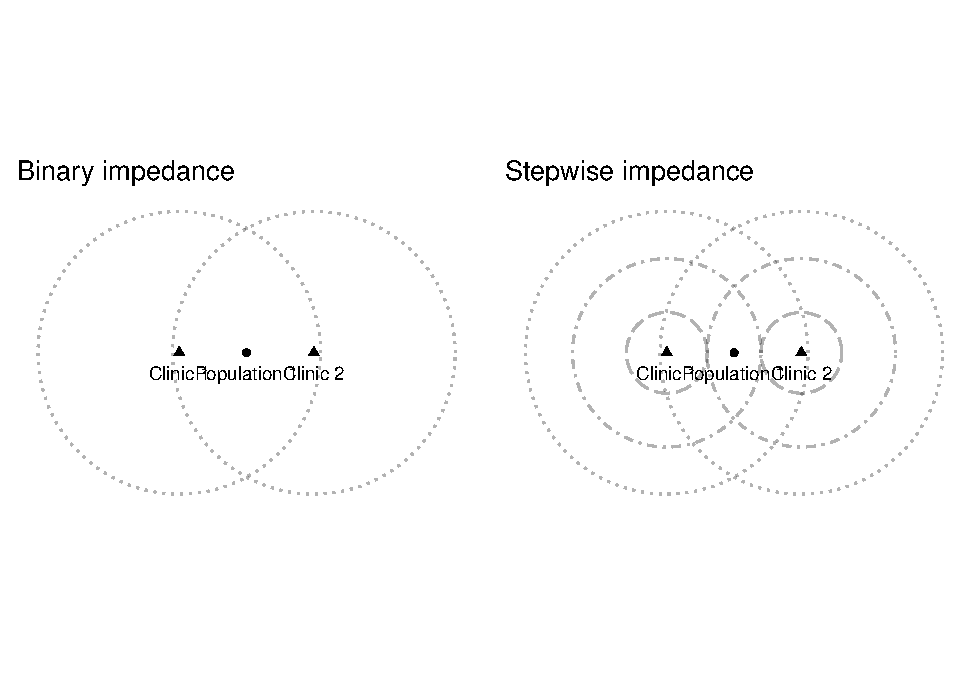
\includegraphics[width=0.95\linewidth]{Supply_and_Demand_Inflation_in_FCA_Methods_v2.0_files/figure-latex/fig1-example-1-1} \caption{\label{fig:fig1-example-1}A single population center that enters the service areas of two clinics (triangles are clinics, dotted lines are segments of catchment areas)}\label{fig:fig1-example-1}
\end{figure}

Clearly, only when the full population at \(i\) is allocated exclusively
to one service point (i.e., when \(K_i=1\)) the implied demand equals
the population - something that seldom happens in practical situations.

It is important to acknowledge that demand in accessibility analysis
represents the \emph{potential} for spatial interaction, not realized
interaction. That said, the expectation that facilities need to serve
multiple times the size of the population in a region can easily lead to
misleading conclusions about the need for resources. A logical question,
however, is whether the inflation of demand (with the consequence
deflation of level of service) is not offset in the second step of the
method, when the population at \(i\) has potential access to multiple
service points?

Let us consider what happens in the second step of the algorithm in the
example, when catchment areas are floated to the population center (see
Fig \ref{fig:fig2-example-2}). When a binary impedance function is used,
the aggregation of the level of service means that, despite the
inflation of demand due to double-counting, accessibility matches the
level of service \emph{as well as} the regional PPR of \(2/100\) (left
panel). In the case of the stepwise function, the level of implied
demand is less than the population, but the population is also assumed
to receive less of the available level of service. In this case, again,
the accessibility matches the level of service \emph{despite the fact
that segments of the population were assumed to not contribute to
demand}.

\begin{figure}
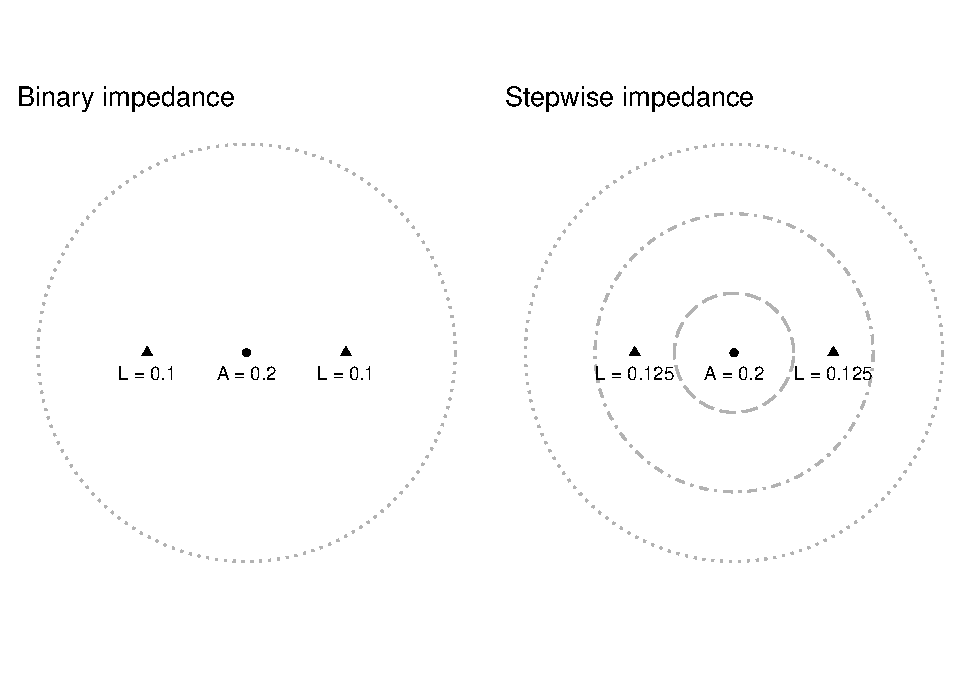
\includegraphics[width=0.95\linewidth]{Supply_and_Demand_Inflation_in_FCA_Methods_v2.0_files/figure-latex/fig2-example-2-1} \caption{\label{fig:fig2-example-2}Levels of service of three clinics and accessibility of one population center (triangles are clinics, dotted lines are segments of catchment areas)}\label{fig:fig2-example-2}
\end{figure}

Clearly, the example is too simplistic (in fact just a variation of the
container approach), and it is unclear what the implications would be
for a system with even just a slightly more complex geography. To
explore this, consider the addition of two population centers to the
landscape (see Fig \ref{fig:fig3-example-3}). Notice how the three
population centers are in the catchment areas of the two clinics. When
the binary impedance function is used, demand at each clinic is
calculated as \(300\), and demand over all clinics is therefore 600, or
twice the population of the region. When the stepwise impedance function
is used, the demand by each center is: \[
\begin{array}{c}
D_{1j} = 0.8\times 100 + 0.8 \times 100 = 160\\
D_{2j} = 0.8\times 100 + 0.4 \times 100 = 120\\
D_{3j} = 0.4\times 100 + 0.8 \times 100 = 120
\end{array}
\] and the total load on the system is therefore \(400\), still well in
excess of the total population of the region.

When demand is used to calculate the level of service, and then
accessibility in the second step of the algorithm, the following occurs
(see Fig \ref{fig:fig4-example-4}). When the binary impedance function
is used (left panel), the level of service at each clinic is: \[
\begin{array}{c}
L_1 = \frac{10}{300} = 0.033\\
L_2 = \frac{10}{300} = 0.033
\end{array}
\] The level of service at the clinics is only half of the regional PPR,
since each clinic is assumed to serve the \emph{entire} population of
the region. Unfortunately, since demand has been inflated for each
clinic, these levels of service cannot be meaningfully interpreted as
local PPRs. The sum over the clinics, on the other hand, is \(20/300\) -
which is consistent with the regional PPR. Interestingly, as seen in the
figure, the accessibility of each population center matches the regional
PPR - but the sum of accessibility over all population centers exceeds
the sum of the level of service over all the clinics as a consequence of
allocating the same level of service to several population centers.

Continuing with the stepwise impedance function, we can see (Fig
\ref{fig:fig4-example-4}, right panel) that the levels of service are
calculated as: \[
\begin{array}{c}
L_1 = \frac{10}{0.8\times 100 + 0.8\times 100 + 0.4\times 100} = \frac{10}{200} = 0.05\\
L_2 = \frac{10}{0.8\times 100 + 0.4\times 100 + 0.8\times 100} = \frac{10}{200} = 0.05
\end{array}
\] Notice how the level of service is higher in this case: this is a
consequence of assuming (as the stepwise impedance function does) that
some of the population does \emph{not} demand service. Demand, however,
is still inflated, and interpretation of the levels of service as local
PPRs is still inappropriate. Accessibility is higher for population
center 1 but lower for the two peripheral centers. Furthermore, the sum
of accessibility over all population centers exceeds the sum of the
level of service of all clinics in the region.

\begin{figure}
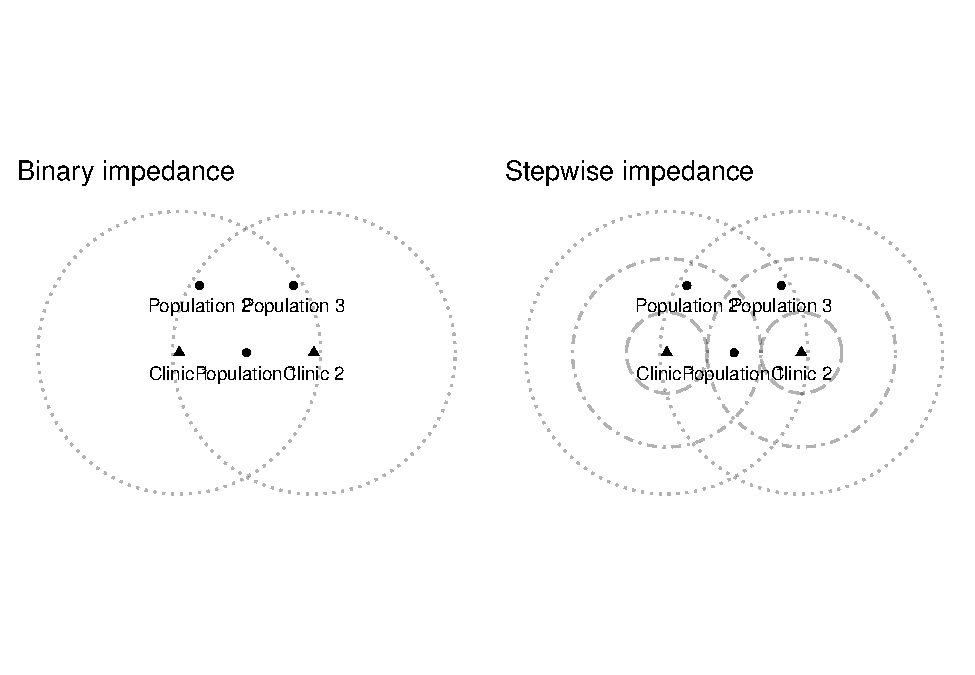
\includegraphics[width=0.95\linewidth]{Supply_and_Demand_Inflation_in_FCA_Methods_v2.0_files/figure-latex/fig3-example-3-1} \caption{\label{fig:fig3-example-3}Three population centers and two clinics (triangles are clinics, dotted lines are segments of catchment areas)}\label{fig:fig3-example-3}
\end{figure}

\begin{figure}
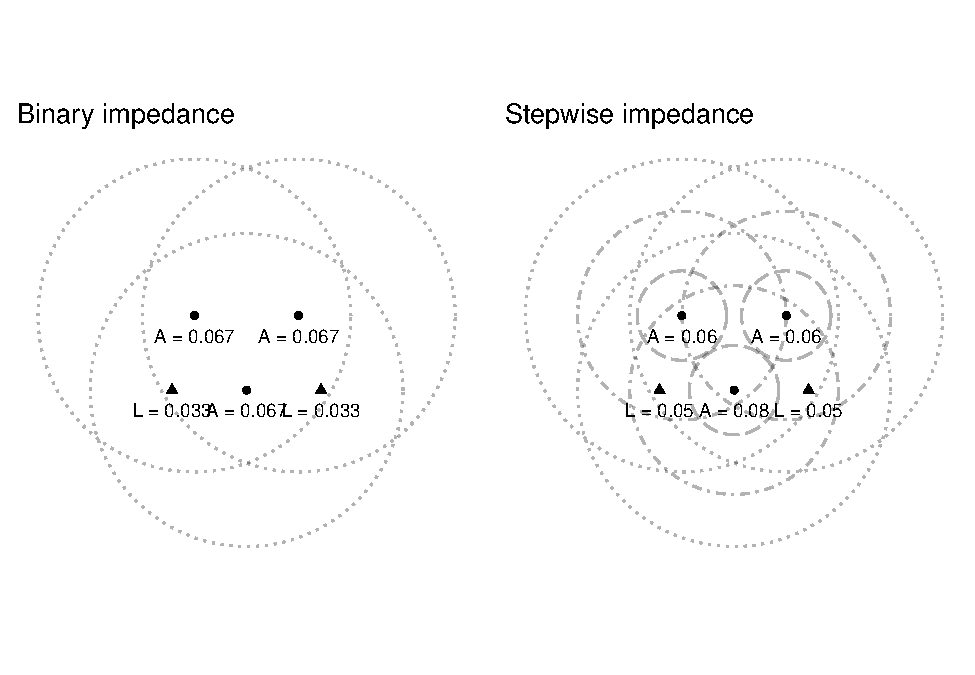
\includegraphics[width=0.95\linewidth]{Supply_and_Demand_Inflation_in_FCA_Methods_v2.0_files/figure-latex/fig4-example-4-1} \caption{\label{fig:fig4-example-4}Levels of service of two clinics and accessibility of three population centers (triangles are clinics, dotted lines are segments of catchment areas)}\label{fig:fig4-example-4}
\end{figure}

At issue is the interpretability of the levels of service, which as the
example illustrates do not accurately represent PPRs, and how
accessibility, which is a weighted sum of levels of service, cannot be
interpreted as the PPR for a population center either.

Two methods reviewed above, namely the Three-Stage Floating Catchment
Area method and the Modified Two-Stage Floating Catchment Area method
aim to address the overestimation of demand and/or levels of service
when calculating accessibility. As discussed previously, they do this by
compounding the effect of the impedance function. In the case of 3SFCA,
demand is deflated by assuming that demand declines more rapidly with
distance. Then, when calculating accessibility, the levels of service
are allocated more locally, again, as a consequence of steeper
distance-decay. In the case of M2SFCA, demand is not deflated, however,
the levels of service are allocated more locally as a consequence of
steeper distance-decay. In other words, these methods correct for
inflation by assuming that \emph{fewer} people demand helath care
services, and that the levels of service are allocated to fewer people
too.

For comparison, the levels of service and accessibility for the example
according to these two methods are shown in Fig
\ref{fig:fig5-example-5}. Notice how the levels of service in the 3FSCA
are considerably higher as a consequence of excluding potential users
with a steeper rate of decay. On the other hand, the levels of
accessibility are also lower, as a consequence of allocating service
more locally. The levels of service in the M2SFCA are identical to the
E2SFCA, however, accessibility is lower, again as a result of allocating
service more locally.

\begin{figure}
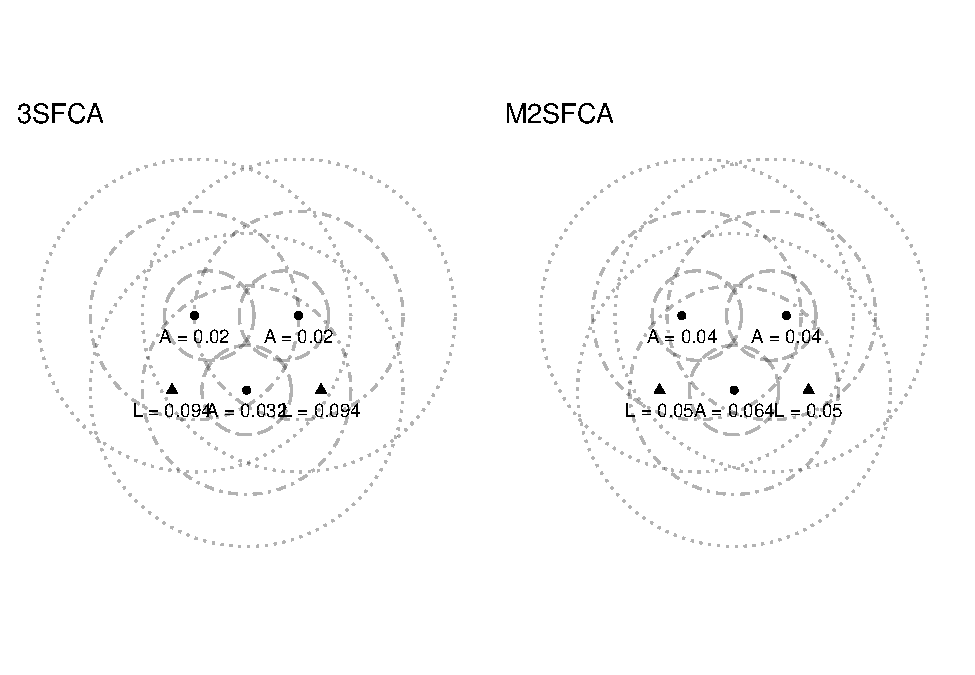
\includegraphics[width=0.95\linewidth]{Supply_and_Demand_Inflation_in_FCA_Methods_v2.0_files/figure-latex/fig5-example-5-1} \caption{\label{fig:fig5-example-5}Levels of service and accessibility according to 3SFCA and M2SFCA methods (triangles are clinics, dotted lines are segments of catchment areas)}\label{fig:fig5-example-5}
\end{figure}

\section{A Simulated Example}\label{a-simulated-example}

The examples in the preceding section illustrate the way demand and
level of service can be overestimaged (and in some cases underestimated)
in FCA algorithms. However, they are too simplistic to indicate what
would happen in a realistic situation. In particular, it is possible
that the consequences depend on the geography of the problem as the
examples in Delamater {[}18{]} suggest. Based on the way demand and
level of service are allocated, we conjecture that the effects are
likely more pronounced in areas with higher density of population and
service, since inflation is a consequence of overlapping catchment
areas. Furthermore, we conjecture that demand inflation will be reduced
when stepwise/continuous distance-decay functions are used, since their
effect is to reduce the overlap by reducing the contribution of
population at different distances, and to allocate levels of service
more locally as well. We explore these issues further by means of a
simple but realistic simulated example.

The setup for the simulated example is shown in Fig
\ref{fig:fig6-simulation}. There are three clinics and nine population
centers. Assume that the supply at the three clinics is one physician at
clinic 1, three physicians at clinic 2, and two physicians at clinic 3.
Further, assume that the population at \(1\), \(2\), \(8\), and \(9\) is
\(250\); population at \(3\), \(4\), and \(6\) is \(250\); and
population at \(5\) and \(7\) is \(1000\). The total population in the
region therefore is \(4,500\). Under this setup, the level of service
across the whole system is \(1.33\) physicians per thousand people,
which we will refer to as the Regional PPR.

\begin{figure}
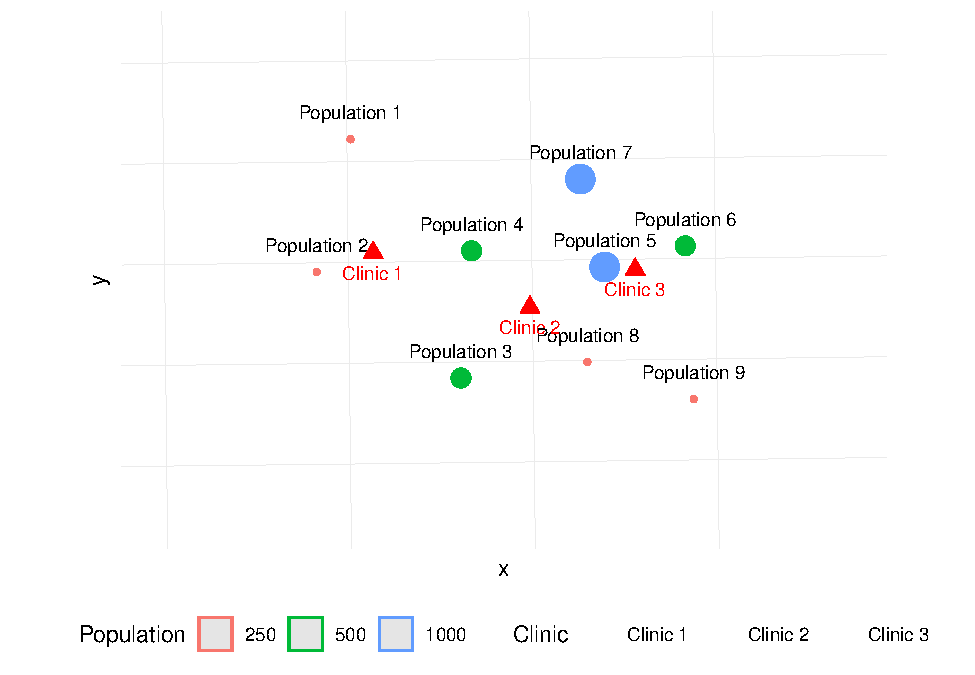
\includegraphics[width=0.95\linewidth]{Supply_and_Demand_Inflation_in_FCA_Methods_v2.0_files/figure-latex/fig6-simulation-1} \caption{\label{fig:fig6-simulation}Setup for the simulation exercise}\label{fig:fig6-simulation}
\end{figure}

For this experiment, we consider binary and stepwise impedance
functions. The former is simply the traditional 2SFCA method, whereas
the latter is the Enhanced 2SFCA approach. The catchment areas for the
first step of the algorithm (demand allocation) are shown in Fig
\ref{fig:fig7a-simulation-step1} (binary impedance) and Fig Fig
\ref{fig:fig7b-simulation-step1} (stepwise impedance). Notice that some
population centers are inside the catchment areas of more than one
clinic. For instance, Population Center 5 is in the catchment areas of
Clinics 2 and 3, whereas Population Center 4 is in the catchment areas
of all three clinics.

\begin{figure}
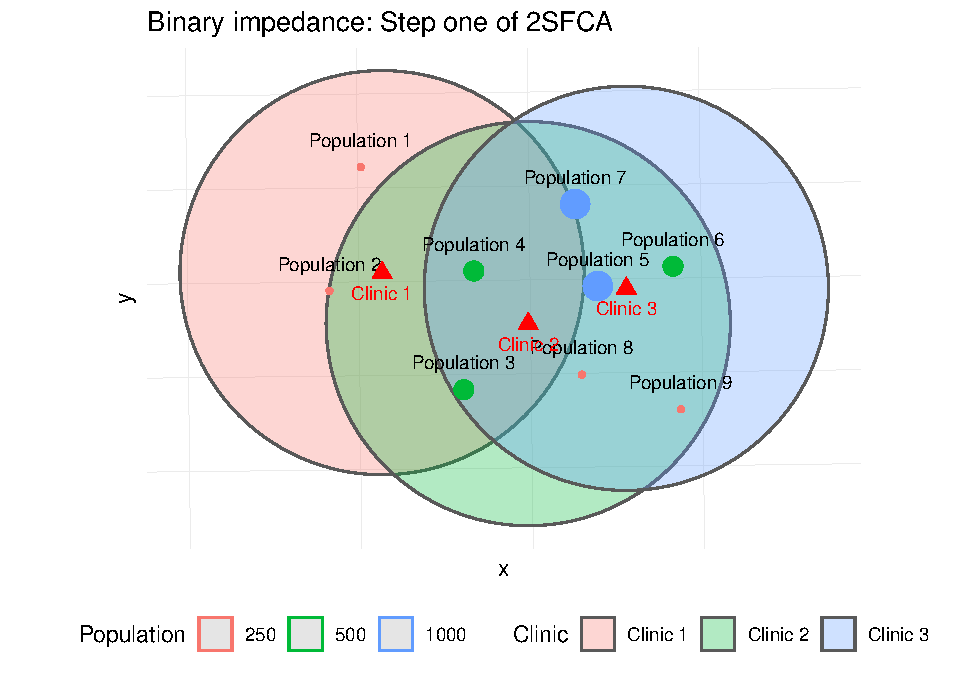
\includegraphics[width=0.95\linewidth]{Supply_and_Demand_Inflation_in_FCA_Methods_v2.0_files/figure-latex/fig7a-simulation-step1-1} \caption{\label{fig:fig7a-simulation-step1}Catchment areas in step 1, according to binary and stepwise impedance functions (the weights of the stepwise function are 0.945, 0.600, and 0.424)}\label{fig:fig7a-simulation-step1}
\end{figure}

\begin{figure}
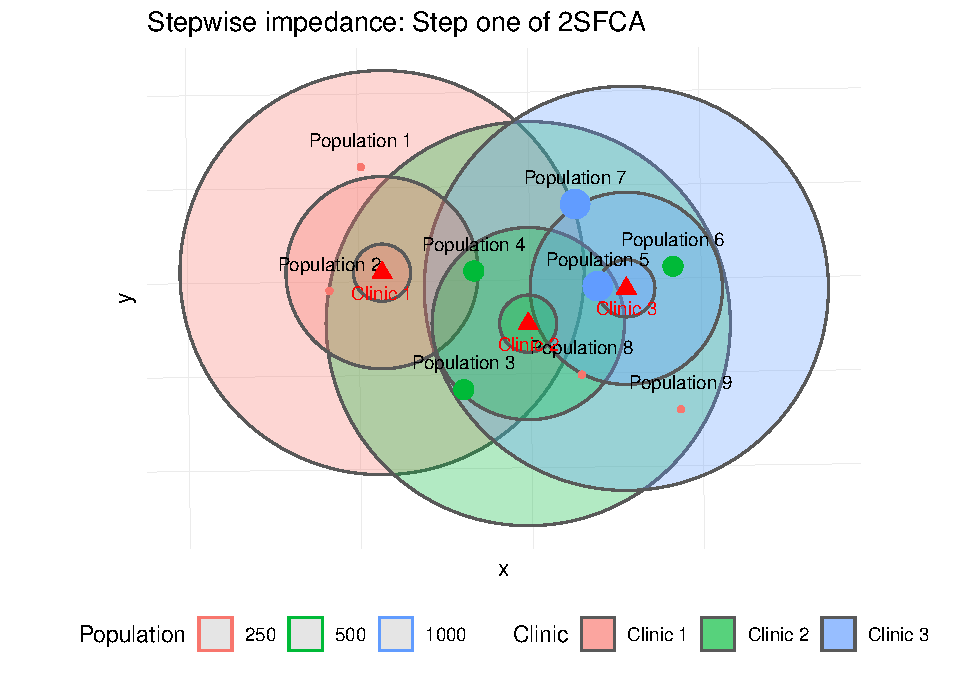
\includegraphics[width=0.95\linewidth]{Supply_and_Demand_Inflation_in_FCA_Methods_v2.0_files/figure-latex/fig7b-simulation-step1-1} \caption{\label{fig:fig7b-simulation-step1}Catchment areas in step 1, according to binary and stepwise impedance functions (the weights of the stepwise function are 0.945, 0.600, and 0.424)}\label{fig:fig7b-simulation-step1}
\end{figure}

To see how the overlap of catchment areas impacts the calculations in
the first step of the algorithm, we define impedance matrices using the
same criteria as for the buffers seen in Fig
\ref{fig:fig7-simulation-step1}. These matrices are shown in Table
\ref{tab:table-simulation-impedance}.

\begin{table}[t]

\caption{\label{tab:table-simulation-impedance}\label{tab:table-simulation-step1-impedance}Impedance Matrices and Step 1 of the FCA Algorithm}
\centering
\fontsize{7}{9}\selectfont
\begin{tabular}{lrrrrrr}
\toprule
\multicolumn{1}{c}{ } & \multicolumn{3}{c}{Binary Impedance} & \multicolumn{3}{c}{Stepwise Impedance} \\
\cmidrule(l{2pt}r{2pt}){2-4} \cmidrule(l{2pt}r{2pt}){5-7}
Population Center & Clinic 1 & Clinic 2 & Clinic 3 & Clinic 1 & Clinic 2 & Clinic 3\\
\midrule
Population 1 & 1 & 0 & 0 & 0.242 & 0.000 & 0.000\\
Population 2 & 1 & 1 & 0 & 0.600 & 0.242 & 0.000\\
Population 3 & 1 & 1 & 1 & 0.242 & 0.600 & 0.242\\
Population 4 & 1 & 1 & 1 & 0.600 & 0.600 & 0.242\\
Population 5 & 0 & 1 & 1 & 0.000 & 0.600 & 0.945\\
\addlinespace
Population 6 & 0 & 1 & 1 & 0.000 & 0.242 & 0.600\\
Population 7 & 0 & 1 & 1 & 0.000 & 0.242 & 0.242\\
Population 8 & 0 & 1 & 1 & 0.000 & 0.600 & 0.242\\
Population 9 & 0 & 1 & 1 & 0.000 & 0.242 & 0.242\\
\bottomrule
\end{tabular}
\end{table}

The demand for each clinic is calculated as the population of the
centers multiplied by the values of the corresponding impedance weight
with respect to that clinic, and then aggregated for all population
centers. The level of service is the supply divided by the demand,
multiplied by \(1,000\). The last row of the table shows the total
population as well as the total demand at each clinic.

\begin{landscape}\begin{table}[t]

\caption{\label{tab:table-simulation-demand}\label{tab:table-simulation-demand}Disaggregated Demand Allocations by Population Center and Clinic, and level of Service by Clinic}
\centering
\fontsize{7}{9}\selectfont
\begin{tabular}{lrllllllllllll}
\toprule
\multicolumn{2}{c}{ } & \multicolumn{3}{c}{Binary Impedance} & \multicolumn{3}{c}{Stepwise Impedance} & \multicolumn{3}{c}{3SFCA} & \multicolumn{3}{c}{M2SFCA} \\
\cmidrule(l{2pt}r{2pt}){3-5} \cmidrule(l{2pt}r{2pt}){6-8} \cmidrule(l{2pt}r{2pt}){9-11} \cmidrule(l{2pt}r{2pt}){12-14}
Population Center & Population & Clinic 1 & Clinic 2 & Clinic 3 & Clinic 1 & Clinic 2 & Clinic 3 & Clinic 1 & Clinic 2 & Clinic 3 & Clinic 1 & Clinic 2 & Clinic 3\\
\midrule
Population 1 & 250 & \textcolor[HTML]{0D0887}{250} & \textcolor[HTML]{FCCE25}{0} & \textcolor[HTML]{FCCE25}{0} & \textcolor[HTML]{EF7D50}{60.5} & \textcolor[HTML]{FCCE25}{0} & \textcolor[HTML]{FCCE25}{0} & \textcolor[HTML]{EF7D50}{60.5} & \textcolor[HTML]{FCCE25}{0} & \textcolor[HTML]{FCCE25}{0} & \textcolor[HTML]{EF7D50}{60.5} & \textcolor[HTML]{FCCE25}{0} & \textcolor[HTML]{FCCE25}{0}\\
Population 2 & 250 & \textcolor[HTML]{0D0887}{250} & \textcolor[HTML]{0D0887}{250} & \textcolor[HTML]{FCCE25}{0} & \textcolor[HTML]{A51F99}{150} & \textcolor[HTML]{EF7D50}{60.5} & \textcolor[HTML]{FCCE25}{0} & \textcolor[HTML]{CE4B75}{106.89} & \textcolor[HTML]{FDB42F}{17.388} & \textcolor[HTML]{FCCE25}{0} & \textcolor[HTML]{A51F99}{150} & \textcolor[HTML]{EF7D50}{60.5} & \textcolor[HTML]{FCCE25}{0}\\
Population 3 & 500 & \textcolor[HTML]{0D0887}{500} & \textcolor[HTML]{0D0887}{500} & \textcolor[HTML]{0D0887}{500} & \textcolor[HTML]{F58A47}{121} & \textcolor[HTML]{AB2494}{300} & \textcolor[HTML]{F58A47}{121} & \textcolor[HTML]{FCCE25}{27.013} & \textcolor[HTML]{E76F5A}{166.05} & \textcolor[HTML]{FCCE25}{27.013} & \textcolor[HTML]{F58A47}{121} & \textcolor[HTML]{AB2494}{300} & \textcolor[HTML]{F58A47}{121}\\
Population 4 & 500 & \textcolor[HTML]{0D0887}{500} & \textcolor[HTML]{0D0887}{500} & \textcolor[HTML]{0D0887}{500} & \textcolor[HTML]{A92296}{300} & \textcolor[HTML]{A92296}{300} & \textcolor[HTML]{F3874A}{121} & \textcolor[HTML]{F2844B}{124.83} & \textcolor[HTML]{F2844B}{124.83} & \textcolor[HTML]{FCCE25}{20.307} & \textcolor[HTML]{A92296}{300} & \textcolor[HTML]{A92296}{300} & \textcolor[HTML]{F3874A}{121}\\
Population 5 & 1000 & \textcolor[HTML]{FCCE25}{0} & \textcolor[HTML]{0D0887}{1000} & \textcolor[HTML]{0D0887}{1000} & \textcolor[HTML]{FCCE25}{0} & \textcolor[HTML]{A51F99}{600} & \textcolor[HTML]{2B0594}{945} & \textcolor[HTML]{FCCE25}{0} & \textcolor[HTML]{F0804E}{233.01} & \textcolor[HTML]{AB2494}{578.01} & \textcolor[HTML]{FCCE25}{0} & \textcolor[HTML]{A51F99}{600} & \textcolor[HTML]{2B0594}{945}\\
\addlinespace
Population 6 & 500 & \textcolor[HTML]{FCCE25}{0} & \textcolor[HTML]{0D0887}{500} & \textcolor[HTML]{0D0887}{500} & \textcolor[HTML]{FCCE25}{0} & \textcolor[HTML]{EF7D50}{121} & \textcolor[HTML]{A51F99}{300} & \textcolor[HTML]{FCCE25}{0} & \textcolor[HTML]{FDB42F}{34.777} & \textcolor[HTML]{CE4B75}{213.78} & \textcolor[HTML]{FCCE25}{0} & \textcolor[HTML]{EF7D50}{121} & \textcolor[HTML]{A51F99}{300}\\
Population 7 & 1000 & \textcolor[HTML]{FCCE25}{0} & \textcolor[HTML]{0D0887}{1000} & \textcolor[HTML]{0D0887}{1000} & \textcolor[HTML]{FCCE25}{0} & \textcolor[HTML]{EF7D50}{242} & \textcolor[HTML]{EF7D50}{242} & \textcolor[HTML]{FCCE25}{0} & \textcolor[HTML]{FCA238}{121} & \textcolor[HTML]{FCA238}{121} & \textcolor[HTML]{FCCE25}{0} & \textcolor[HTML]{EF7D50}{242} & \textcolor[HTML]{EF7D50}{242}\\
Population 8 & 250 & \textcolor[HTML]{FCCE25}{0} & \textcolor[HTML]{0D0887}{250} & \textcolor[HTML]{0D0887}{250} & \textcolor[HTML]{FCCE25}{0} & \textcolor[HTML]{A51F99}{150} & \textcolor[HTML]{EF7D50}{60.5} & \textcolor[HTML]{FCCE25}{0} & \textcolor[HTML]{CE4B75}{106.89} & \textcolor[HTML]{FDB42F}{17.388} & \textcolor[HTML]{FCCE25}{0} & \textcolor[HTML]{A51F99}{150} & \textcolor[HTML]{EF7D50}{60.5}\\
Population 9 & 250 & \textcolor[HTML]{FCCE25}{0} & \textcolor[HTML]{0D0887}{250} & \textcolor[HTML]{0D0887}{250} & \textcolor[HTML]{FCCE25}{0} & \textcolor[HTML]{EF7D50}{60.5} & \textcolor[HTML]{EF7D50}{60.5} & \textcolor[HTML]{FCCE25}{0} & \textcolor[HTML]{FCA238}{30.25} & \textcolor[HTML]{FCA238}{30.25} & \textcolor[HTML]{FCCE25}{0} & \textcolor[HTML]{EF7D50}{60.5} & \textcolor[HTML]{EF7D50}{60.5}\\
Total Population/Demand & 4500 & 1500 & 4250 & 4000 & 631.5 & 1834 & 1850 & 319.228 & 834.191 & 1007.744 & 631.5 & 1834 & 1850\\
\addlinespace
Supply & NA & 1 & 3 & 2 & 1 & 3 & 2 & 1 & 3 & 2 & 1 & 3 & 2\\
Level of Service (per 1,000) & NA & 0.667 & 0.706 & 0.5 & 1.584 & 1.636 & 1.081 & 3.133 & 3.596 & 1.985 & 1.584 & 1.636 & 1.081\\
\bottomrule
\multicolumn{14}{l}{\textit{Note: }}\\
\multicolumn{14}{l}{Darker number colors in a row indicate a greater allocation of demand. }\\
\end{tabular}
\end{table}
\end{landscape}

First we discuss the results according to the binary impedance function.
As seen in Table \ref{tab:table-simulation-demand}, the population of
Center 3 (which is in the catchment area of three clinics) is assumed to
contribute \(1,500\) patients to the demand across the system, whereas
Center 1 (which is in the catchment area of only one clinic) contributes
exactly its population of \(250\). Since the population of several
centers is counted multiple times, the apparent demand exceeds the
actual population. In effect, when we calculate the total demand (the
sum of the demand across clinics), we find that this is 9,750 according
to the binary impedance function, which far exceeds the actual
population.

Turning now to the stepwise function, we see that Center 3 contributes
\(500 \times 0.242 + 500 \times 0.600 + 500 \times 0.242 = 542\) to the
demand across the system, but Center 1 contributes only
\(250 \times 0.242= 60.5\). The total demand now is 4,316, which is
\emph{less} than the total population.

This example illustrates a vexing effect in how FCA methods operate:
when multiple service points are within the threshold travel cost of a
population center, it is assumed that some (and possibly all) of the
same persons crowd more than one service point, resulting in inflated
demand and deflated levels of service. On the other hand, when stepwise
or continuous functions (e.g., E2SFCA) are used to weigh down the
population of distant population centers, the apparent effect is that
some segments of the population do \emph{not} demand service, even when
clinics are within their threshold travel cost. This effect is even more
marked in the case of 3SFCA, which produces considerably higher levels
of service, as a consequence of stacking the effects of two impedance
functions. In effect, demand is deflated and the level of service is
inflated. While the assumption that some members of the population drop
out from the total demand pool may be acceptable for discretionary
services, it is suspect when it comes to essential services such as many
health care services, and particularly primary health care.

Recall as well that the Regional Average PPR in this example is \(1.33\)
physicians per thousand. If the total implied demand according to the
binary impedance function is \(9,750\) the corresponding PPR is
\(0.615\) physicians per thousand, or about half of the regional ratio.
The corresponding PPR for the stepwise impedance function (implied
demand = \(4315.5\)) is \(1.39\) physicians per thousand, much closer to
the Regional Average PPR. However, this PPR is misleading in that it
assumes that some segments of the population are served multiple times,
and some are not served at all.

Clearly, the first step of the algorithm can lead to inflation or
deflation of the levels of demand. But do these matter? Or do they
somehow average out when the levels of service are aggregated in the
second step of the algorithm? Again, the situation is not clear-cut when
multiple population centers and/or service clinics interact through
overlapping catchment areas.

To illustrate this, we proceed to estimate the accessibility for the
example using the binary and the stepwise impedance matrices. The
results appear in Table \ref{tab:table-simulation-los-accessibility}.

\begin{landscape}\begin{table}[t]

\caption{\label{tab:table-simulation-los-accessibility}\label{tab:table-simulation-los-accessibility}Disaggregated Level of Service Allocations by Clinic and Population Center, and Accessibility by Population Center}
\centering
\fontsize{7}{9}\selectfont
\begin{tabular}{lrrrlllllllll}
\toprule
Clinic & Supply & Demand & Level of Service & Center 1 & Center 2 & Center 3 & Center 4 & Center 5 & Center 6 & Center 7 & Center 8 & Center 9\\
\midrule
\addlinespace[0.3em]
\multicolumn{13}{l}{\textbf{Binary Impedance}}\\
\hspace{1em}1 & 1 & 1500.000 & 0.667 & \textcolor[HTML]{46039F}{0.667} & \textcolor[HTML]{DE5E65}{0.667} & \textcolor[HTML]{F3854B}{0.667} & \textcolor[HTML]{F3874A}{0.667} & \textcolor[HTML]{FCCE25}{0} & \textcolor[HTML]{FCCE25}{0} & \textcolor[HTML]{FCCE25}{0} & \textcolor[HTML]{FCCE25}{0} & \textcolor[HTML]{FCCE25}{0}\\
\hspace{1em}2 & 3 & 4250.000 & 0.706 & \textcolor[HTML]{FCCE25}{0} & \textcolor[HTML]{D9586A}{0.706} & \textcolor[HTML]{F07F4F}{0.706} & \textcolor[HTML]{F0804E}{0.706} & \textcolor[HTML]{E26660}{0.706} & \textcolor[HTML]{A92296}{0.706} & \textcolor[HTML]{A92296}{0.706} & \textcolor[HTML]{E26660}{0.706} & \textcolor[HTML]{A92296}{0.706}\\
\hspace{1em}3 & 2 & 4000.000 & 0.500 & \textcolor[HTML]{FCCE25}{0} & \textcolor[HTML]{FCCE25}{0} & \textcolor[HTML]{FBA139}{0.5} & \textcolor[HTML]{FCA238}{0.5} & \textcolor[HTML]{F0804E}{0.5} & \textcolor[HTML]{D24F71}{0.5} & \textcolor[HTML]{D24F71}{0.5} & \textcolor[HTML]{F0804E}{0.5} & \textcolor[HTML]{D24F71}{0.5}\\
\hspace{1em}Accessibility & NA & NA & NA & \textcolor[HTML]{46039F}{0.667} & \textcolor[HTML]{7B02A8}{1.37} & \textcolor[HTML]{5102A3}{1.87} & \textcolor[HTML]{5601A4}{1.87} & \textcolor[HTML]{B02991}{1.21} & \textcolor[HTML]{0D0887}{1.21} & \textcolor[HTML]{0D0887}{1.21} & \textcolor[HTML]{B02991}{1.21} & \textcolor[HTML]{0D0887}{1.21}\\
\addlinespace[0.3em]
\multicolumn{13}{l}{\textbf{Stepwise Impedance}}\\
\hspace{1em}1 & 1 & 631.500 & 1.584 & \textcolor[HTML]{BD3886}{0.383} & \textcolor[HTML]{BD3886}{0.95} & \textcolor[HTML]{FDB52E}{0.383} & \textcolor[HTML]{DD5E66}{0.95} & \textcolor[HTML]{FCCE25}{0} & \textcolor[HTML]{FCCE25}{0} & \textcolor[HTML]{FCCE25}{0} & \textcolor[HTML]{FCCE25}{0} & \vphantom{1} \textcolor[HTML]{FCCE25}{0}\\
\hspace{1em}2 & 3 & 1834.000 & 1.636 & \textcolor[HTML]{FCCE25}{0} & \textcolor[HTML]{F3874A}{0.396} & \textcolor[HTML]{D8576B}{0.981} & \textcolor[HTML]{DA5A6A}{0.981} & \textcolor[HTML]{C9447A}{0.981} & \textcolor[HTML]{E26660}{0.396} & \textcolor[HTML]{E26660}{0.396} & \textcolor[HTML]{C9447A}{0.981} & \vphantom{1} \textcolor[HTML]{E26660}{0.396}\\
\hspace{1em}3 & 2 & 1850.000 & 1.081 & \textcolor[HTML]{FCCE25}{0} & \textcolor[HTML]{FCCE25}{0} & \textcolor[HTML]{FCCC25}{0.262} & \textcolor[HTML]{FCCE25}{0.262} & \textcolor[HTML]{C6417E}{1.02} & \textcolor[HTML]{B52F8C}{0.649} & \textcolor[HTML]{F3854B}{0.262} & \textcolor[HTML]{FCA238}{0.262} & \vphantom{1} \textcolor[HTML]{F3854B}{0.262}\\
\hspace{1em}Accessibility & NA & NA & NA & \textcolor[HTML]{BD3886}{0.383} & \textcolor[HTML]{8004A8}{1.35} & \textcolor[HTML]{7E03A8}{1.63} & \textcolor[HTML]{0D0887}{2.19} & \textcolor[HTML]{330597}{2} & \textcolor[HTML]{4D02A1}{1.04} & \textcolor[HTML]{B42E8D}{0.657} & \textcolor[HTML]{AC2694}{1.24} & \textcolor[HTML]{B42E8D}{0.657}\\
\addlinespace[0.3em]
\multicolumn{13}{l}{\textbf{3SFCA}}\\
\hspace{1em}1 & 1 & 319.228 & 3.133 & \textcolor[HTML]{0D0887}{0.758} & \textcolor[HTML]{0D0887}{1.88} & \textcolor[HTML]{EB7655}{0.758} & \textcolor[HTML]{5502A4}{1.88} & \textcolor[HTML]{FCCE25}{0} & \textcolor[HTML]{FCCE25}{0} & \textcolor[HTML]{FCCE25}{0} & \textcolor[HTML]{FCCE25}{0} & \textcolor[HTML]{FCCE25}{0}\\
\hspace{1em}2 & 3 & 834.191 & 3.596 & \textcolor[HTML]{FCCE25}{0} & \textcolor[HTML]{C7427C}{0.87} & \textcolor[HTML]{0D0887}{2.16} & \textcolor[HTML]{18068B}{2.16} & \textcolor[HTML]{0D0887}{2.16} & \textcolor[HTML]{8004A8}{0.87} & \textcolor[HTML]{8004A8}{0.87} & \textcolor[HTML]{0D0887}{2.16} & \textcolor[HTML]{8004A8}{0.87}\\
\hspace{1em}3 & 2 & 1007.744 & 1.985 & \textcolor[HTML]{FCCE25}{0} & \textcolor[HTML]{FCCE25}{0} & \textcolor[HTML]{FCA438}{0.48} & \textcolor[HTML]{FCA537}{0.48} & \textcolor[HTML]{4903A0}{1.88} & \textcolor[HTML]{18068B}{1.19} & \textcolor[HTML]{D5546E}{0.48} & \textcolor[HTML]{F1834C}{0.48} & \textcolor[HTML]{D5546E}{0.48}\\
\hspace{1em}Accessibility & NA & NA & NA & \textcolor[HTML]{FDB32F}{0.0551} & \textcolor[HTML]{F58C46}{0.367} & \textcolor[HTML]{FCCE25}{0.253} & \textcolor[HTML]{FA9C3C}{0.536} & \textcolor[HTML]{EF7D50}{0.525} & \textcolor[HTML]{FA9C3C}{0.17} & \textcolor[HTML]{FEBE2A}{0.0514} & \textcolor[HTML]{FDAE32}{0.198} & \textcolor[HTML]{FEBE2A}{0.0514}\\
\addlinespace[0.3em]
\multicolumn{13}{l}{\textbf{M2SFCA}}\\
\hspace{1em}1 & 1 & 631.500 & 1.584 & \textcolor[HTML]{BD3886}{0.383} & \textcolor[HTML]{BD3886}{0.95} & \textcolor[HTML]{FDB52E}{0.383} & \textcolor[HTML]{DD5E66}{0.95} & \textcolor[HTML]{FCCE25}{0} & \textcolor[HTML]{FCCE25}{0} & \textcolor[HTML]{FCCE25}{0} & \textcolor[HTML]{FCCE25}{0} & \textcolor[HTML]{FCCE25}{0}\\
\hspace{1em}2 & 3 & 1834.000 & 1.636 & \textcolor[HTML]{FCCE25}{0} & \textcolor[HTML]{F3874A}{0.396} & \textcolor[HTML]{D8576B}{0.981} & \textcolor[HTML]{DA5A6A}{0.981} & \textcolor[HTML]{C9447A}{0.981} & \textcolor[HTML]{E26660}{0.396} & \textcolor[HTML]{E26660}{0.396} & \textcolor[HTML]{C9447A}{0.981} & \textcolor[HTML]{E26660}{0.396}\\
\hspace{1em}3 & 2 & 1850.000 & 1.081 & \textcolor[HTML]{FCCE25}{0} & \textcolor[HTML]{FCCE25}{0} & \textcolor[HTML]{FCCC25}{0.262} & \textcolor[HTML]{FCCE25}{0.262} & \textcolor[HTML]{C6417E}{1.02} & \textcolor[HTML]{B52F8C}{0.649} & \textcolor[HTML]{F3854B}{0.262} & \textcolor[HTML]{FCA238}{0.262} & \textcolor[HTML]{F3854B}{0.262}\\
\hspace{1em}Accessibility & NA & NA & NA & \textcolor[HTML]{FCA238}{0.0927} & \textcolor[HTML]{DE5E65}{0.666} & \textcolor[HTML]{ED7953}{0.745} & \textcolor[HTML]{BF3984}{1.22} & \textcolor[HTML]{8004A8}{1.55} & \textcolor[HTML]{D5536F}{0.485} & \textcolor[HTML]{FB9F3A}{0.159} & \textcolor[HTML]{E66C5C}{0.652} & \textcolor[HTML]{FB9F3A}{0.159}\\
\bottomrule
\multicolumn{13}{l}{\textit{Note: }}\\
\multicolumn{13}{l}{Darker number colors in a column indicate a greater allocation of level of service or accessibility. }\\
\end{tabular}
\end{table}
\end{landscape}

Accessibility in the table is calculated as the level of service of the
clinics multiplied by the the values of the impedance function with
respect to a population center, and then aggregated for all clinics. As
seen in the table, the levels of accessibility vary considerably
depending on the method. As anticipated, use of non-binary impedance
functions reduces the inflation effect, and can even lead to deflation.
Consider for instance the case of the binary impedance matrix: the total
level of service in the system is the sum of the level of service at the
three clinics, or 1.87. The level of service \emph{allocated} to
population centers, on the other hand, is the sum of the accessibility
in the system, or 11.8. When using the stepwise impedance function, the
total level of service in the system is 4.3, and the level of service
allocated to population centers is 11.2. Compare this to the case of
3SFCA, where the total level of service in the system is 8.71, but the
level of service allocated to population centers is only 2.21; or the
case of M2SFCA, which estimates the total level of service in the system
as 4.3 (same as E2SFCA) but allocates 5.74 to population centers.

Clearly, all the methods give qualitatively similar results, with
peripheral centers displaying lower accessibility and more central
places higher. But there are important differences in how demand and
level of service are allocated throughout the system to calculate
accessibilty. Figure \ref{fig:fig-comparison} shows how the different
methods penalize peripheral centers at different rates. And, since the
demand is not consistent with the population and the accessibility is
not consistent with the level of service of the clinics, it is difficult
to interpret the results in terms PPRs. For instance, when we inspect
the results for the binary impedance matrix (2SFCA), we can see in the
table that the accessibility of Population Center 1 is simply the level
of service of Clinic 1. But, as we saw before, this level of service was
deflated by double counting the population of Centers 2, 3, and 4, which
contribute to the calculation of demand at multiple clinics. Things
become more complex as the number of overlapping catchment areas grows.
For example, Population Center 2 contributed to the congestion effect of
two clinics. However, demand at one of those clinics was calculated
using the population of eight out of nine population centers. What this
suggests is that, at the very least, some population centers (likely
those in the periphery of regions) will have artificially low
accessibility levels as a consequence of demand inflation.

\begin{figure}
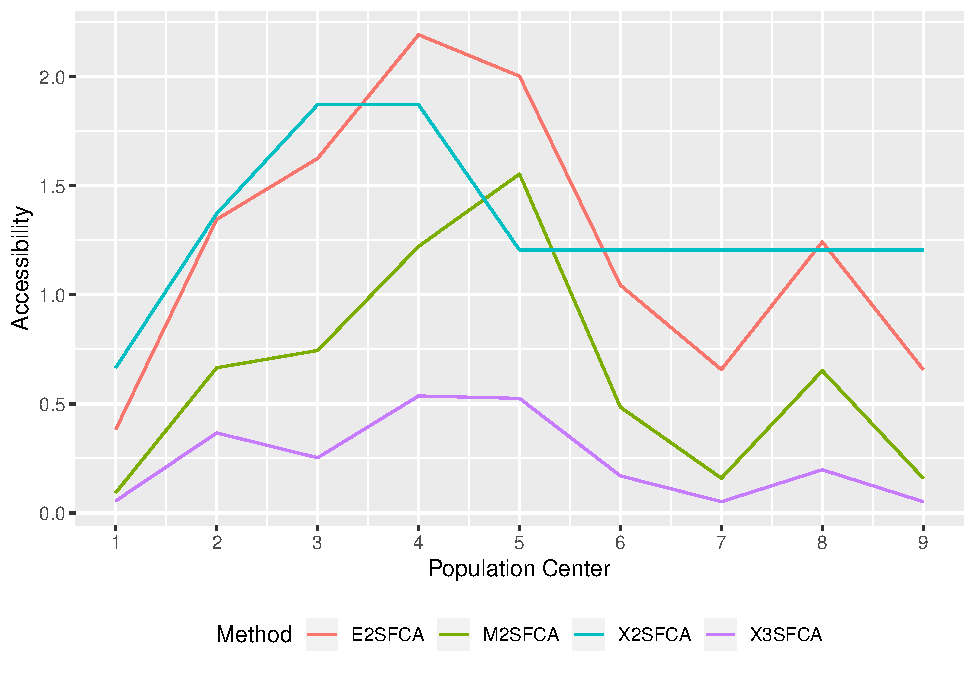
\includegraphics[width=0.95\linewidth]{Supply_and_Demand_Inflation_in_FCA_Methods_v2.0_files/figure-latex/fig-comparison-1} \caption{\label{fig:fig-comparison}Accessibility by Population Center by Method}\label{fig:fig-comparison}
\end{figure}

\section{A Method for Proportional Allocation of Demand and
Supply}\label{a-method-for-proportional-allocation-of-demand-and-supply}

As the examples in the preceding subsection illustrate, FCA methods can
induce quite substantial inflation (or deflation) of demand and level of
service. This, in turn, can affect the estimates of accessibility in
potentially complex ways. The results, furthermore lack a clear
interpretation. In this section, we propose a simple and intuitive
adjustment to avoid the inflation artifacts inherent in current
implementations of FCA methods.

Refer again to Fig \ref{fig:fig1-example-1}. Demand inflation occurs
because of the overlap in catchment areas - with the underlying
assumption that a service location services the population within its
catchment area. More realistically, only a fraction of that population
will demand service at the location if other service points are within
reach (i.e., inside its ``floated'' catchment area).

For instance, assuming (as the binary impedance function does), that
individuals at Population Center \(1\) are indifferent between Clinics
\(1\) and \(2\), then it is reasonable to think that the population will
sort itself proportionally to these two clinics - in this example, this
means that half of the population will attend one of two different
clinics (importantly, this assumes that the services on offer are
undifferentiated; one would not generally consider cancer screening and
hair removal clinics competitors). This suggests the following
adjustment to the way the level of demand is calculated. Given an
impedance function, a set of adjusted weights, say \(W^{i*}_{ij}\), are
precalculated by dividing the original impedance weights by the sum of
the weights for population center \(i\) over all service points \(j\):
\[
W_{ij}^{i} = \frac{W_{ij}}{\sum_j W_{ij}}
\]

Please notice that these weights are identical to the selection weights
of the 3SFCA method. A key property of the adjusted weights is the
following: \[
\sum_jW_{ij}^{i}=1
\]

This adjustment procedure has the effect that, when the level of demand
of \(i\) is summed over all service points \(j\), the aggregated level
of demand due to \(i\) is identical to its population: \[
\sum_j P_iW_{ij}^{i} = P_i
\]

As a result of standardizing the impedance weights, population is
allocated \emph{proportionally} to clinics.

On the supply side, inflation happens because the level of service
available at location \(j\) is assumed to be available to every
population center \(i\) within its catchment area. To adjust this,
another set of weights, say \(W^{j*}_{ij}\), is pre-calculated by
dividing the original impedance weights \(W_{ij}\) by the sum of the
weights for service point \(j\) over all population centers \(i\): \[
W_{ij}^{j} = \frac{W_{ij}}{\sum_i W_{ij}}
\]

Again, the resulting weights have the property that: \[
\sum_iW_{ij}^{j}=1
\]

As before, the result of this procedure is that, when the level of
service of \(j\) is aggregated by population centers, the total level of
service for that service point is preserved: \[
\sum_i L_jW_{ij}^{j} = L_j 
\]

Note that, since the weights add up to one, they can be interpreted as a
\emph{probability} or \emph{frequency} of contact, similar to the Huff
model of {[}19{]}.

In reference to Fig \ref{fig:fig3-example-3} (left panel), we can see
that the original binary (unadjusted) weights for Population Centre
\(1\) are \(W_{11} = 1\), \(W_{12} = 1\), the weights of population
center \(2\) are \(W_{21} = 1\), \(W_{22} = 1\), and the weights of
population center \(3\) are \(W_{31} = 1\), \(W_{32} = 1\).

On the demand side, the adjusted weights become for Population Center
\(1\), \(W^{i}_{11} = 1/2\), \(W^{i}_{12} = 1/2\), for Population Center
\(2\) \(W^{i}_{21} = 1/2\), \(W^{i}_{22} = 1/2\), and for Population
Center \(3\) \(W^{i}_{31} = 1/2\), \(W^{i}_{32} = 1/2\). Using the
adjusted weights, it can be seen that the level of demand due to each
population center equals its respective population: \[
\begin{array}{ll}
            \sum_j D_1j = 1/2P_1 + 1/2P_1 = P_1\\
            \sum_j D_2j = 1/2P_2 + 1/2P_2 = P_2\\
            \sum_j D_3j = 1/2P_3 + 1/2P_3 = P_3
        \end{array}
\]

Coming next to the supply side, the adjusted weights for Clinic \(1\)
are \(W^{j*}_{11} = 1/3\), \(W^{i*}_{21} = 1/3\), and
\(W^{i*}_{23} = 1/3\); for Clinic \(2\) the adjusted weights are
\(W^{j*}_{12} = 1/3\), \(W^{i*}_{22} = 1/3\), and \(W^{i*}_{32} = 1/3\).
It can be seen that the level of service is preserved across clinics,
and therefore across the system: \[
\begin{array}{ll}
            \sum_i L_{i1} = L_{1}/3 + L_{1}/3 + L_{1}/3 = L_1\\
            \sum_i L_{i2} = L_{2}/3 + L_{2}/3 + L_{2}/3 = L_2
        \end{array}
\]

The method to adjust the weights used above is identical to a procedure
that will be familiar to readers acquainted with the literature in the
fields of spatial statistics and econometrics. The same adjustment is
widely used there under the names of row- and column-standardization of
a weights matrix {[}24,25{]}.

The proposed adjustment can be easily implemented. We will present next
the implementation using a compact matrix notation. Begin by defining
the following impedance matrix: \[
\mathbf{W} = \left(\begin{array}{ccc}
            W_{11} & \cdots & W_{1J}\\
            \vdots & \ddots & \vdots\\
            W_{N1} & \cdots & W_{NJ}\\
        \end{array}
        \right)
\] where \(W_{ij}\) is an impedance function evaluated at \(d_{ij}\).
Subindex \(i\) is for population centers (\(i=1,\dots,N\)) and subindex
\(j\) is for service points (\(j=1,\dots,J\)). Note that the matrix does
not need to be square. A row-standardized set of weights is obtained as
follows: \[
\mathbf{W}^{i} = \left(\begin{array}{ccc}
            \frac{W_{11}}{\sum_jW_{1j}} & \cdots & \frac{W_{1J}}{\sum_jW_{1j}}\\
            \vdots & \ddots & \vdots\\
            \frac{W_{N1}}{\sum_jW_{Nj}} & \cdots & \frac{W_{NJ}}{\sum_jW_{Nj}}\\
        \end{array}
        \right)
\]

Next, a column-standardized set of weights is calculated as: \[
\mathbf{W}^{j} = \left(\begin{array}{ccc}
            \frac{W_{11}}{\sum_iW_{i1}} & \cdots & \frac{W_{1J}}{\sum_iW_{iJ}}\\
            \vdots & \ddots & \vdots\\
            \frac{W_{N1}}{\sum_iW_{i1}} & \cdots & \frac{W_{NJ}}{\sum_iW_{iJ}}\\
        \end{array}
        \right)
\]

In the first example above (see Fig \ref{fig:fig1-example-1}), the
binary impedance matrix is: \[
\mathbf{W}_{binary} = \left(\begin{array}{ccc}
            1 & 1\\
            1 & 1\\
            1 & 1\\
        \end{array}
        \right)
\]

The row-standardized weights that correspond to this matrix are: \[
\mathbf{W}^{i}_{binary} = \left(\begin{array}{ccc}
            1/2 & 1/2\\
            1/2 & 1/2\\
            1/2 & 1/2\\
        \end{array}
        \right)
\] and the column-standardized weights are: \[
\mathbf{W}^{j}_{binary} = \left(\begin{array}{ccc}
            1/3 & 1/3\\
            1/3 & 1/3\\
            1/3 & 1/3\\
        \end{array}
        \right)
\]

The stepwise impedance weights in the example are: \[
\mathbf{W}_{stepwise} = \left(\begin{array}{ccc}
            0.8 & 0.8\\
            0.8 & 0.4\\
            0.4 & 0.8\\
        \end{array}
        \right)
\]

The row-standardized weights in turn are: \[
\mathbf{W}^{i}_{stepwise} = \left(\begin{array}{ccc}
            1/2 & 1/2\\
            2/3 & 1/3\\
            1/3 & 2/3\\
        \end{array}
        \right)
\] whereas the column-standardized weights are: \[
\mathbf{W}^{j}_{stepwise} = \left(\begin{array}{ccc}
            4/10 & 4/10\\
            4/10 & 2/10\\
            2/10 & 4/10\\
        \end{array}
        \right)
\]

Once that the impedance weights have been adjusted, a vector of adjusted
level of demand \(\mathbf{D}^*\) can be obtained by multiplying the
\emph{transposed} impedance matrix by a vector of population values as
follows: \[
\mathbf{D}^* = [\mathbf{W}^{i}]^T\mathbf{P}
\] where the \(^T\) operator is for ``transpose'', and \(\mathbf{P}\)
is: \[
\mathbf{P} = \left(\begin{array}{c}
            P_1\\
            \vdots\\
            P_N\\
        \end{array}
        \right) 
\]

The level of demand for the service points in the binary impedance
function example is (in vector form): \[
\mathbf{D}^*_{binary}= \left( \begin{array}{ccc}
1/2 & 1/2 & 1/2\\
1/2 & 1/2 & 1/2\\
\end{array} \right)
\left( \begin{array}{c}
100\\
100\\
100
\end{array} \right)=
\left( \begin{array}{c}
300/2\\
300/2\\
\end{array} \right)=
\left( \begin{array}{c}
150\\
150\\
\end{array} \right)
\] Notice how each clinic is expected to service only \(150\), and the
level of demand over the system is identical to the total population.

The level of demand for the service points in the stepwise impedance
function example is (in vector form): \[
\mathbf{D}^*_{sw}= \left( \begin{array}{ccc}
1/2 & 2/3 & 1/3\\
1/2 & 1/3 & 2/3\\
\end{array} \right)
\left( \begin{array}{c}
100\\
100\\
100
\end{array} \right)=
\left( \begin{array}{c}
50 + 200/3 + 100/3\\
50 + 100/3 + 200/3
\end{array} \right)=
\left( \begin{array}{c}
150\\
150
\end{array} \right)
\] As can be seen, the aggregated level of demand, after the adjustment,
equals (as desired) the actual population of the region. In the case of
the stepwise function, total demand has been adjusted to the population
of the region without the restrictive assumption that some people are
excluded from the system. This is achieved by assuming an assortative
process that leads to proportional allocation of the demand.

The levels of demand can then be used to calculate the level of service
at the individual clinic locations by performing Hadamard division
(\(\oslash\)) of the vector of supply by the vector of adjusted demand.
This is the first step of the 2SFCA (aggregating demand over catchment
areas for service points): \[
\mathbf{L}^* = \mathbf{S}\oslash\mathbf{D}^*
\]

Since Hadamard division is an element-by-element operation, the adjusted
levels of service in the first example (using the binary impedance
function) are:

\[
\mathbf{L}^*_{b} = \left( \begin{array}{c}
10 \\
10 \\
\end{array}\right)\oslash
\left( \begin{array}{c}
150\\
150\\
\end{array} \right)=
\left( \begin{array}{c}
10/150\\
10/150\\
\end{array} \right)=
\left( \begin{array}{c}
0.067\\
0.067\\
\end{array} \right)
\]

The levels of service in the second example, when using the stepwise
impedance function, are also: \[
\mathbf{L}^*_{sw} = \left( \begin{array}{c}
10 \\
10 \\
\end{array}\right)\oslash
\left( \begin{array}{c}
150\\
150\\
\end{array} \right)=
\left( \begin{array}{c}
10/150\\
10/150\\
\end{array} \right)=
\left( \begin{array}{c}
0.067\\
0.067\\
\end{array} \right)
\]

Unlike the 2SFCA, E2SFCA, and 3SFCA methods that produce levels of
service that resemble PPRs but with values that are inconsistent with
total demand given the population, this operation returns values that
are genuinely local PPRs that are consistent with the population of the
region. As we saw above, the demand equals the population. Here, the
supply also equals the number of physicians in the region. Because both
demand and supply are not inflated or deflated in this rectified method,
these values are easily interpretable relative to the Regional Average
PPR of \(20/300\) or \(0.067\) physicians per person. In the case of the
example, it is clear that both clinics have PPRs that are identical to
the Regional Average PPR.

Accessibility, finally, is calculated as the matrix product of the
column-standardized weights and the adjusted level of service: \[
\mathbf{A}^*=\mathbf{W}^{j}\mathbf{L}^*
\] which, continuing with the example, gives the following for the
binary impedance function: \[
\mathbf{A}^*_{b} = 
\left(\begin{array}{ccc}
1/3 & 1/3\\
1/3 & 1/3\\
1/3 & 1/3\\
        \end{array}
        \right)
\left( \begin{array}{c}
10/150\\
10/150\\
\end{array} \right) =
\left( \begin{array}{c}
10/450 + 10/450\\
10/450 + 10/450\\
10/450 + 10/450\\
\end{array} \right)=
\left( \begin{array}{c}
0.044\\
0.044\\
0.044
\end{array} \right)
\] Notice how the sum of accessibility over the region is consistent
with the total level of service over all clinics (i.e., 0.133). The
level of service has been allocated in its totality.

When using the stepwise impedance function, accessibility is calculated
as: \[
\mathbf{A}^*_{sw} = 
\left(\begin{array}{ccc}
4/10 & 4/10\\
4/10 & 2/10\\
2/10 & 4/10\\
\end{array} \right)
\left( \begin{array}{c}
10/150\\
10/150\\
\end{array} \right) =
\left( \begin{array}{c}
4/150 + 4/150\\
4/150 + 2/150\\
2/150 + 4/150
\end{array} \right)=
\left( \begin{array}{c}
0.053\\
0.040\\
0.040
\end{array} \right)
\] Again, the sum of accessibility is consistent with the level of
service available from all clinics in the region. As with the Local
PPRs, accessibility is interpreted as population-to-provider ratios for
each population center in such a way that all calculations are with
total demand and total level of service. In particular, accessibility
can be interpreted as the share of level of service that a population
center receives from all the clinics that service it.

For the sake of comparison, levels of service and accessibility are
reported for the simulated example in Tables
\ref{tab:table-simulation-demand-adjusted} and
\ref{tab:table-simulation-los-accessibility-adjusted}.

\begin{landscape}\begin{table}[t]

\caption{\label{tab:table-simulation-demand-adjusted}\label{tab:table-simulation-demand-adjusted}Disaggregated Proportional Demand Allocations by Population Center and Clinic, and level of Service by Clinic, using Adjusted Weights}
\centering
\fontsize{7}{9}\selectfont
\begin{tabular}{lrllllll}
\toprule
\multicolumn{2}{c}{ } & \multicolumn{3}{c}{Binary Impedance - Adjusted} & \multicolumn{3}{c}{Stepwise Impedance - Adjusted} \\
\cmidrule(l{2pt}r{2pt}){3-5} \cmidrule(l{2pt}r{2pt}){6-8}
Population Center & Population & Clinic 1 & Clinic 2 & Clinic 3 & Clinic 1 & Clinic 2 & Clinic 3\\
\midrule
Population 1 & 250 & \textcolor[HTML]{0D0887}{250} & \textcolor[HTML]{FCCE25}{0} & \textcolor[HTML]{FCCE25}{0} & \textcolor[HTML]{0D0887}{250} & \textcolor[HTML]{FCCE25}{0} & \textcolor[HTML]{FCCE25}{0}\\
Population 2 & 250 & \textcolor[HTML]{8505A7}{125} & \textcolor[HTML]{8505A7}{125} & \textcolor[HTML]{FCCE25}{0} & \textcolor[HTML]{0D0887}{178.15} & \textcolor[HTML]{D45270}{71.853} & \textcolor[HTML]{FCCE25}{0}\\
Population 3 & 500 & \textcolor[HTML]{E16462}{166.67} & \textcolor[HTML]{E16462}{166.67} & \textcolor[HTML]{E16462}{166.67} & \textcolor[HTML]{FCCE25}{111.62} & \textcolor[HTML]{0D0887}{276.75} & \textcolor[HTML]{FCCE25}{111.62}\\
Population 4 & 500 & \textcolor[HTML]{900DA4}{166.67} & \textcolor[HTML]{900DA4}{166.67} & \textcolor[HTML]{900DA4}{166.67} & \textcolor[HTML]{0D0887}{208.04} & \textcolor[HTML]{0D0887}{208.04} & \textcolor[HTML]{FCCE25}{83.911}\\
Population 5 & 1000 & \textcolor[HTML]{FCCE25}{0} & \textcolor[HTML]{5C01A6}{500} & \textcolor[HTML]{5C01A6}{500} & \textcolor[HTML]{FCCE25}{0} & \textcolor[HTML]{9A169F}{388.35} & \textcolor[HTML]{0D0887}{611.65}\\
\addlinespace
Population 6 & 500 & \textcolor[HTML]{FCCE25}{0} & \textcolor[HTML]{8505A7}{250} & \textcolor[HTML]{8505A7}{250} & \textcolor[HTML]{FCCE25}{0} & \textcolor[HTML]{D45270}{143.71} & \textcolor[HTML]{0D0887}{356.29}\\
Population 7 & 1000 & \textcolor[HTML]{FCCE25}{0} & \textcolor[HTML]{0D0887}{500} & \textcolor[HTML]{0D0887}{500} & \textcolor[HTML]{FCCE25}{0} & \textcolor[HTML]{0D0887}{500} & \textcolor[HTML]{0D0887}{500}\\
Population 8 & 250 & \textcolor[HTML]{FCCE25}{0} & \textcolor[HTML]{8505A7}{125} & \textcolor[HTML]{8505A7}{125} & \textcolor[HTML]{FCCE25}{0} & \textcolor[HTML]{0D0887}{178.15} & \textcolor[HTML]{D45270}{71.853}\\
Population 9 & 250 & \textcolor[HTML]{FCCE25}{0} & \textcolor[HTML]{0D0887}{125} & \textcolor[HTML]{0D0887}{125} & \textcolor[HTML]{FCCE25}{0} & \textcolor[HTML]{0D0887}{125} & \textcolor[HTML]{0D0887}{125}\\
Total Population/Demand & 4500 & 708.333 & 1958.333 & 1833.333 & 747.815 & 1891.852 & 1860.333\\
\addlinespace
Supply & NA & 1 & 3 & 2 & 1 & 3 & 2\\
Level of Service (per 1,000) & NA & 1.412 & 1.532 & 1.091 & 1.337 & 1.586 & 1.075\\
\bottomrule
\multicolumn{8}{l}{\textit{Note: }}\\
\multicolumn{8}{l}{Darker number colors in a row indicate a greater allocation of demand. }\\
\end{tabular}
\end{table}
\end{landscape}

\begin{landscape}\begin{table}[t]

\caption{\label{tab:table-simulation-los-accessibility-adjusted}\label{tab:table-simulation-los-accessibility-adjusted}Disaggregated Proportional Level of Service Allocations by Clinic and Population Center, and Accessibility by Population Center, using Adjusted Weights}
\centering
\fontsize{7}{9}\selectfont
\begin{tabular}{lrrrlllllllll}
\toprule
Clinic & Supply & Demand & Level of Service & Center 1 & Center 2 & Center 3 & Center 4 & Center 5 & Center 6 & Center 7 & Center 8 & Center 9\\
\midrule
\addlinespace[0.3em]
\multicolumn{13}{l}{\textbf{Binary Impedance - Adjusted}}\\
\hspace{1em}1 & 1 & 708.333 & 1.412 & \textcolor[HTML]{0D0887}{0.353} & \textcolor[HTML]{A51F99}{0.353} & \textcolor[HTML]{CE4B75}{0.353} & \textcolor[HTML]{DF6263}{0.353} & \textcolor[HTML]{FCCE25}{0} & \textcolor[HTML]{FCCE25}{0} & \textcolor[HTML]{FCCE25}{0} & \textcolor[HTML]{FCCE25}{0} & \textcolor[HTML]{FCCE25}{0}\\
\hspace{1em}2 & 3 & 1958.333 & 1.532 & \textcolor[HTML]{FCCE25}{0} & \textcolor[HTML]{E26660}{0.191} & \textcolor[HTML]{F9963F}{0.191} & \textcolor[HTML]{FBA238}{0.191} & \textcolor[HTML]{E76F5A}{0.191} & \textcolor[HTML]{B32B8E}{0.191} & \textcolor[HTML]{B32B8E}{0.191} & \textcolor[HTML]{BD3886}{0.191} & \textcolor[HTML]{B32B8E}{0.191}\\
\hspace{1em}3 & 2 & 1833.333 & 1.091 & \textcolor[HTML]{FCCE25}{0} & \textcolor[HTML]{FCCE25}{0} & \textcolor[HTML]{FCA934}{0.156} & \textcolor[HTML]{FDB030}{0.156} & \textcolor[HTML]{F07F4F}{0.156} & \textcolor[HTML]{CB4679}{0.156} & \textcolor[HTML]{CA457A}{0.156} & \textcolor[HTML]{D14E72}{0.156} & \textcolor[HTML]{CA457A}{0.156}\\
\hspace{1em}Accessibility & NA & NA & NA & \textcolor[HTML]{0D0887}{0.353} & \textcolor[HTML]{350498}{0.544} & \textcolor[HTML]{0D0887}{0.7} & \textcolor[HTML]{6300A7}{0.7} & \textcolor[HTML]{B6308B}{0.347} & \textcolor[HTML]{100788}{0.347} & \textcolor[HTML]{0D0887}{0.347} & \textcolor[HTML]{350498}{0.347} & \textcolor[HTML]{0D0887}{0.347}\\
\addlinespace[0.3em]
\multicolumn{13}{l}{\textbf{Stepwise Impedance - Adusted}}\\
\hspace{1em}1 & 1 & 747.815 & 1.337 & \textcolor[HTML]{B32D8E}{0.192} & \textcolor[HTML]{6001A6}{0.476} & \textcolor[HTML]{F9963F}{0.192} & \textcolor[HTML]{BE3885}{0.476} & \textcolor[HTML]{FCCE25}{0} & \textcolor[HTML]{FCCE25}{0} & \textcolor[HTML]{FCCE25}{0} & \textcolor[HTML]{FCCE25}{0} & \textcolor[HTML]{FCCE25}{0}\\
\hspace{1em}2 & 3 & 1891.852 & 1.586 & \textcolor[HTML]{FCCE25}{0} & \textcolor[HTML]{F58C46}{0.114} & \textcolor[HTML]{E56A5D}{0.282} & \textcolor[HTML]{EF7C51}{0.282} & \textcolor[HTML]{CE4A75}{0.282} & \textcolor[HTML]{E26561}{0.114} & \textcolor[HTML]{E26561}{0.114} & \textcolor[HTML]{7501A8}{0.282} & \textcolor[HTML]{E26561}{0.114}\\
\hspace{1em}3 & 2 & 1860.333 & 1.075 & \textcolor[HTML]{FCCE25}{0} & \textcolor[HTML]{FCCE25}{0} & \textcolor[HTML]{FCCE25}{0.0944} & \textcolor[HTML]{FCCE25}{0.0944} & \textcolor[HTML]{AD2793}{0.369} & \textcolor[HTML]{8E0DA4}{0.234} & \textcolor[HTML]{EB7556}{0.0944} & \textcolor[HTML]{EE7B51}{0.0944} & \textcolor[HTML]{EB7556}{0.0944}\\
\hspace{1em}Accessibility & NA & NA & NA & \textcolor[HTML]{B32D8E}{0.192} & \textcolor[HTML]{0D0887}{0.59} & \textcolor[HTML]{6800A8}{0.569} & \textcolor[HTML]{0D0887}{0.853} & \textcolor[HTML]{0D0887}{0.651} & \textcolor[HTML]{0D0887}{0.348} & \textcolor[HTML]{A51F99}{0.208} & \textcolor[HTML]{0D0887}{0.377} & \textcolor[HTML]{A51F99}{0.208}\\
\bottomrule
\multicolumn{13}{l}{\textit{Note: }}\\
\multicolumn{13}{l}{Darker number colors in a column indicate a greater allocation of level of service or accessibility. }\\
\end{tabular}
\end{table}
\end{landscape}

An important point to remark is the following. The use of row- and
column-standardized impedance weights assumes that the full population
of every population center within the catchment of a clinic will receive
service. However, the allocation, although proportional, is different
when binary or stepwise impedance weights are standardized. When binary
weights are employed, the underlying idea is that potential for use is
identical within the catchment area irrespective of distance. When
stepwise weights are used, proportionally more of the population is
allocated to closer clinics. Depending on the definition of cost of
travel, this allows a research to accommodate directional effects as
well. For example, use of network travel time would tend to favor
movement away from congested locations.

\subsection{Suboptimal Systems}\label{suboptimal-systems}

The research of Delamater {[}18{]} illustrates how accessibility
estimates can be misleading when systems are not optimally configured.
We understand this to mean that some population centers are located too
far away from service points to actually benefit from them. In the
modified 2SFCA method (M2SFCA), Delamater addresses this issue by
increasing the friction of distance. A slight inconsistency in this
approach is that some of the centers that contribute to demand fail to
benefit from the service due to the increased friction to which the
allocation of the level of service is subjected. Our suggestion in the
case of suboptimal systems is to use an impedance function that reflects
limiting conditions. For instance, in urban settings a travel time
longer than 2 hours might be considered too long to be serviced by any
clinic.

\subsection{System Efficiency}\label{system-efficiency}

The approach proposed in this paper allocates population and level of
service proportionally and exactly. This assumes that the population
sorts itself into clinics in the most efficient way. But what if some
members of the population lack full information about the spatial
distribution of clinics? Or have some bias towards centric locations?
The vagaries of human behavior could create excess demand in some
locations, and as a consequence supply surpluses in others. Situations
like this can be accommodated in a relatively straightforward way using
our approach.

Here, we describe the use of \emph{slack factors}. Demand and level of
service are allocated proportionally and exhaustively (i.e., 100\%). But
the standardization could allow for some slack, by inflating demand
and/or supply in a controlled way.

Our proposal to standardize the weights was as follows, for the case of
rows and columns respectively: \[
\mathbf{W}^{i} = \left(\begin{array}{ccc}
            \frac{W_{11}}{\sum_jW_{1j}} & \cdots & \frac{W_{1J}}{\sum_jW_{1j}}\\
            \vdots & \ddots & \vdots\\
            \frac{W_{N1}}{\sum_jW_{Nj}} & \cdots & \frac{W_{NJ}}{\sum_jW_{Nj}}\\
        \end{array}
        \right)
\text{  and  }
\mathbf{W}^{j} = \left(\begin{array}{ccc}
            \frac{W_{11}}{\sum_iW_{i1}} & \cdots & \frac{W_{1J}}{\sum_iW_{iJ}}\\
            \vdots & \ddots & \vdots\\
            \frac{W_{N1}}{\sum_iW_{i1}} & \cdots & \frac{W_{NJ}}{\sum_iW_{iJ}}\\
        \end{array}
        \right)
\]

A set of slack factors, say \(k^i_i\), could be introduced in the
following manner: \[
\mathbf{W}^{i} = \left(\begin{array}{ccc}
            \frac{k^i_1W_{11}}{\sum_jW_{1j}} & \cdots & \frac{k^i_1W_{1J}}{\sum_jW_{1j}}\\
            \vdots & \ddots & \vdots\\
            \frac{k^i_NW_{N1}}{\sum_jW_{Nj}} & \cdots & \frac{k^i_NW_{NJ}}{\sum_jW_{Nj}}\\
        \end{array}
        \right)
\] A value of \(k^i_1=1.10\) would inflate the demand of population
center \(i=1\) by 10\%, whereas a value of \(k^i_1 = 1.20\) would
inflate the demand by 20\%. In a similar way, a set of slack factors
\(k^j_i\) could be introduced to modulate the allocation of supply: \[
\mathbf{W}^{j} = \left(\begin{array}{ccc}
            \frac{k^j_1W_{11}}{\sum_iW_{i1}} & \cdots & \frac{k^j_{J}W_{1N_J}}{\sum_iW_{iJ}}\\
            \vdots & \ddots & \vdots\\
            \frac{k^j_{1}W_{N1}}{\sum_iW_{i1}} & \cdots & \frac{k^j_JW_{NJ}}{\sum_iW_{iJ}}\\
        \end{array}
        \right)
\] A value of \(k^j_1=0.9\), for example, would deflate the supply of
clinic \(j=1\) by 10\%. The use of slack factors provides an interesting
way of modulating demand and level of service allocation in a very
precise and controlled way, and presents interesting opportunities as
well to introduce expert opinion or other empirical approaches to
callibrate slack factors.

\section{Empirical Example}\label{empirical-example}

In the reminder of the paper we present an empirical example to
illustrate the application of the methods presented above. Based on the
preceding discussion, the adjusted 2SFCA method employed can be
summarized as: \[
L_{j}=\sum_i\frac{S_j}{P_iW_{ij}^{i}}
\] with row-standardized impedance weights \(W_{ij}^i\) in the first
step, and:

\[
A_i = \sum_j{L_jW_{ij}^{j}}
\] with colum-standardized impedance weights \(W_{ij}^j\) in the second
step. The same approach is used to re-weight the impedance function for
the stepwise approach (i.e., E2SFCA).

The case study is based on accessibility to family physicians in the
Hamilton Census Metropolitan Area (CMA), in Ontario, Canada. For this,
we use data collected about the distribution of the population and
primary health care clinics (i.e., family physicians) in the region.
Time use data from Canada's General Social Survey (GSS) was also used to
inform the selection of thresholds for the impedance functions. The data
collection and preprocessing protocols are described next.

\subsection{Family Physicians and Clinic
Locations}\label{family-physicians-and-clinic-locations}

In regards to the supply of clinics, the locations of family physicians
were obtained using the College of Physicians and Surgeons of Ontario
(CPSO) database for the Province of Ontario. We chose this organization
beacuse all physicians practicing in Ontario are required to register
with the CPSO, as set out in the Ontario Regulation 865/93: Registration
{[}26{]}.

Our search of CPSO's database was conducted attending to the following
criteria.

\begin{enumerate}
\def\labelenumi{\arabic{enumi})}
\item
  Only physicians who are registered as family physicians were selected
  (this excluded specialists such as pediatric physicians).
\item
  The spatial extent of the search was determined using forward
  sortation areas (FSAs), which are the first three initial characters
  of a postal code. Using a GIS, the regions of interest were selected
  by choosing FSAs within a 10 kilometer buffer distance from the
  Hamilton CMA boundary. This involved 72 different FSA regions. Each
  FSA region code was then searched in the CPSO database in addition to
  the family physician specification.
\end{enumerate}

The parameters of the search were deliberately conservative, and the
search identified a total of 2,224 family physicians practicing in the
region, of which, 864 are located in the Hamilton CMA. The resulting
dataset was manually verified by the third author to ensure that the
information was consistent and suitable for geocoding. Prior to
geocoding, locational information was organized in three columns,
containing street address, city name, and province name. After family
physicians were geocoded, locations were further examined. When family
physicians overlapped or were within a 50 meter distance of each other
we merged the records to identify 535 unique locations that we term
``clinics''. Many of these clinics are not in the Hamilton CMA proper,
but provide a buffer to minimize edge effects in the analysis. The
distribution of clinics and family physicians is shown in Fig
\ref{fig:fig8-clinic-map} for the Hamilton CMA.

\begin{figure}
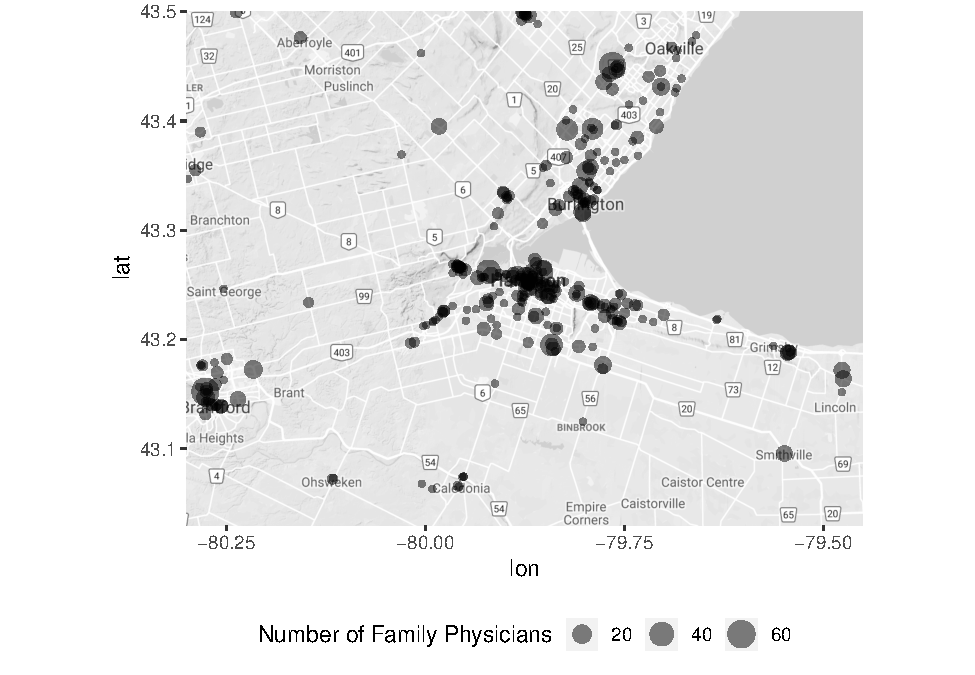
\includegraphics[width=0.95\linewidth]{Supply_and_Demand_Inflation_in_FCA_Methods_v2.0_files/figure-latex/fig8-clinic-map-1} \caption{\label{fig:fig8-clinic-map}Location of clinics and family physicians in the Hamilton CMA and surrounding regions}\label{fig:fig8-clinic-map}
\end{figure}

\subsection{Population}\label{population}

Population information was obtained from the 2011 Canadian Census. To
maximize the spatial resolution, population data were acquired at the
Dissemination Area (DA) level of geography for all DAs within the
selected FSAs. As a result, this includes DAs not in the Hamilton CMA
proper, but that provide a buffer against edge effects. From this, the
region contains a population of 2,959,090, of which 720,725 are in the
Hamilton CMA. The distribution of population in the Hamilton CMA is
shown in Fig \ref{fig:fig9-population-map}.

\begin{figure}
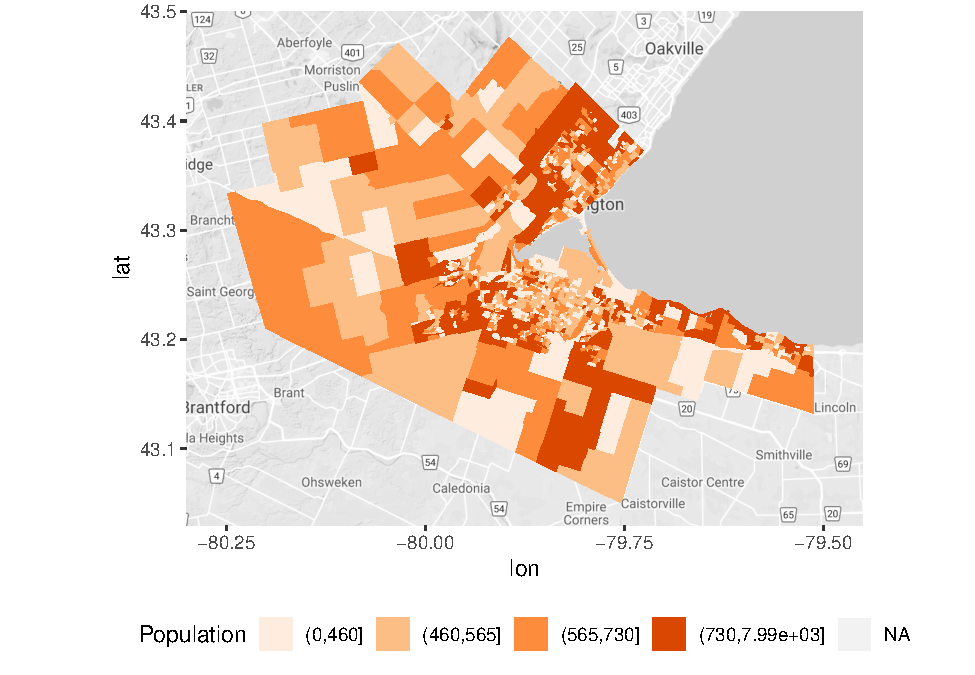
\includegraphics[width=0.95\linewidth]{Supply_and_Demand_Inflation_in_FCA_Methods_v2.0_files/figure-latex/fig9-population-map-1} \caption{\label{fig:fig9-population-map}Population distribution in the Hamilton CMA}\label{fig:fig9-population-map}
\end{figure}

\subsection{Travel Time Matrix}\label{travel-time-matrix}

Calculation of impedance weights requires that we evaluate an impedance
function at values of \(d_ij\), that is, the cost of travel between DA
\(i\) and clinic \(j\). In this research we used travel time as our cost
variable. To this end, we computed a matrix of travel times measured
over the road network. To calculate the travel time between population
centers and clinics we used the DA centroids and the geocoded locations
of clinics. Shortest paths on the network and subsequently travel times
were computed using a Geographic Information System.

\subsection{Impedance Functions}\label{impedance-functions}

For the experiments we use two different impedance functions,
corresponding to the 2SFCA and E2SFCA algorithms. We do not implement
the 3SFCA or the M2SFCA methods because, as noted above, they are
equivalent to using steeper impedances. For the 2SFCA apprach, impedance
is given by a binary function, whereas for E2SFCA it is given by a
stepwise function. The impedance functions require that we define cost
(i.e., travel time) thresholds to implement them. To select the
thresholds, we retrieved time use data from Canada's General Social
Survey Cycle 24 (see http://odesi2.scholarsportal.info/webview/).

From the time use files, we filtered all activity episodes corresponding
to respondents living in CMAs/CAs (metropolitan regions) in Ontario.
Next, we filtered all episodes taking place in a car (as driver) while
traveling for personal care activities for household adults (which
includes traveling to see a doctor) and traveling for shopping or
obtaining services (which includes traveling to go to health clinic or
doctor's office). It is worthwhile noting that travel by car accounts
for over 95\% of trips for the selected purposes in Ontario CMAs/CAs.

Once episodes were filtered by mode of travel and purpose of the trip,
their durations (in minutes) were examined by means of quantile
analysis, using episode weights to ensure the representativeness of the
analysis. From the results, we learned that 50\% of all trips by car for
the aforementioned purposes are less than 15 minutes long, and we
selected this value as the threshold \(d_0\) for the binary function. In
other words, this part of the analysis assumes that any person who has
to travel longer than 15 minutes to reach a clinic is outside its
catchment area. We deem this value appropriate for the scale, density,
and level of congestion of Hamilton CMA.

Quantile analysis of trip durations was also used to calibrate a
Gaussian function with standard deviation set at 15 minutes, to match
the value selected for the binary impedance above. This produced the
following stepwise function, with any trips longer than 45 minutes
assumed to be outside of catchment: \[
W(d_{ij}) = \left\{
        \begin{array}{ll}
            0.946 & \quad d_{ij} \leq 5 \\
            0.801 & \quad 5 < d_{ij} \leq 10 \\
            0.607 & \quad 10 < d_{ij} \leq 15 \\
            0.411 & \quad 15 < d_{ij} \leq 20 \\
            0.135 & \quad 20 < d_{ij} \leq 30 \\
            0.011 & \quad 30 < d_{ij} \leq 45 \\
            0.00 & \quad 45 < d_{ij}
        \end{array}
    \right.
\]

Notice how the stepwise function has weights greater than 0.5 for
\(d_{ij} \leq 15 min\) and less than 0.5 for \(d_{ij} > 15 min\). This
means that it will count fewer people than the binary function when
\(d_{ij} \leq 15 min\), but more when \(d_{ij} > 15 min\).

\subsection{Results}\label{results}

We begin our discussion of the results by noting that with a total
population of the region of 2,959,090 and 2,222 family physicians, the
Regional Average PPR ratio is 0.751 family physicians per 1,000 people.
This value is somewhat lower than the value of 1.16 for Ontario reported
by CIHI {[}27{]} and lower than the 1.20 estimated based on the
population and physician data for the Hamilton CMA, which we attribute
to our conservative search criteria of family physicians in the rest of
the region.

The nominal levels of demand, service, and accessibility are calculated
for the 2SFCA and E2SFCA using both the unadjusted and adjusted
impedance matrices. Table \ref{tab:table-descriptive-statistics}
summarizes the results by each impedance matrix. As seen there, when no
adjustment is made, the nominal demand explodes to several times the
actual population in the region. However, when the impedance weights are
standardized, demand is now only slightly less than the total population
for the region, since the system is not optimal in the sense discussed
by Delamater {[}18{]}, and a small proportion of the population turns
out to be outside of catchment. The nominal demand under binary
impedance is lower due to the stricter catchment area condition (i.e.,
less than 15 minutes), compared to the stepwise function (i.e., less
than 45 minutes). This, in turn, is somewhat lower than the total demand
in the Regional Average PPR, which does not impose catchment area
constraints within the region.

It is clear that the rectified demand leads to results that are
considerably more realistic than the conventional approaches. In
addition to the nominal system-wide demand, this is seen as well when
calculating the regional provider-to-population ratios for each case
(i.e., Family Physicians per 1,000 people). As seen in the table, the
mean levels of service for clinics in the region in the case of the
adjusted binary and stepwise weights are in line with their
corresponding Regional Average PPRs. Since the levels of service in the
case of the adjusted weights can be interpreted as local PPRs, this
indicates that the average clinic offers approximately the same level of
service as the regional system does for the whole population.
Furthermore, the mean accessibility of a DA according to the adjusted
weights is identical to the mean LOS: this is because the LOS is
allocated completely to DAs. The total LOS and accessibility in the
region match when the adjusted weights are used. This is not the case
when the unadjusted weights are used. Clearly, the use of the unadjusted
weights can lead to a substantial amount of accessibility inflation, by
factors as high as five or six times the estimates of the proposed
proportional allocation approach.

These results demonstrate how inflation of the supply (i.e., the level
of service) leads to much higher values of accessibility in the case of
the conventional 2SFCA and E2SFCA methods. The procedure to rectify the
population and level of service, on the other hand, leads to
accessibility outputs that are consistent with the regional population
and overall supply of health care services. This, in turn, makes
interpretation of the output more robust and intuitive.

\begin{landscape}\begin{table}[t]

\caption{\label{tab:table-descriptive-statistics}\label{tab:table-descriptive-statistics}Summary of Results Accessibility Analysis Hamilton CMA}
\centering
\fontsize{7}{9}\selectfont
\begin{tabular}{lrlrrrrr}
\toprule
Case & Supply (Doctors) & Nominal Demand & Regional Average PPR & Mean Level of Service per Clinic & Total Level of Service & Mean Accessibility per DA & Total Accessibility\\
\midrule
Binary & 2222 & 176,244,020 & 0.013 & 0.025 & 14.766 & 5.993 & 3481.709\\
Binary Adjusted & 2222 & 2,861,445 & 0.777 & 1.046 & 607.803 & 1.046 & 607.803\\
Stepwise & 2222 & 209,666,501 & 0.011 & 0.069 & 40.050 & 6.023 & 3499.115\\
Stepwise Adjusted & 2222 & 2,957,095 & 0.751 & 0.879 & 510.663 & 0.879 & 510.663\\
\bottomrule
\end{tabular}
\end{table}
\end{landscape}

Another important issue is that spatial distribution of inflation of
demand and level of service. If inflation happened in a uniform way, the
upward bias in the estimates could to some extent be ignored, as long as
relative differences by location remained relatively constant.
Unfortunately, as seen in Fig
\ref{fig:fig10-map-demand-inflation-binary} and Fig
\ref{fig:fig11-map-demand-inflation-stepwise}, demand inflation is far
from uniform. In fact, inflation of demand tends to happen, as per our
earlier conjecture, in areas with higher population density. Inflation
factors are also substantially higher when the binary impedance function
is used. Since this function lacks a gradual distance-decay mechanism,
it is more generous in terms of counting population serviced. Notice the
magnitude of the inflation factors: since the inflation of demand
depends on the number of overlapping catchment areas, a factor of
\(160\), for instance, would suggest that a clinic is expected to
\emph{simultaneously} serve approximately that number of DAs in the
conventional 2SFCA method, and a proportionally similar number in the
conventional E2SFCA method.

\begin{figure}
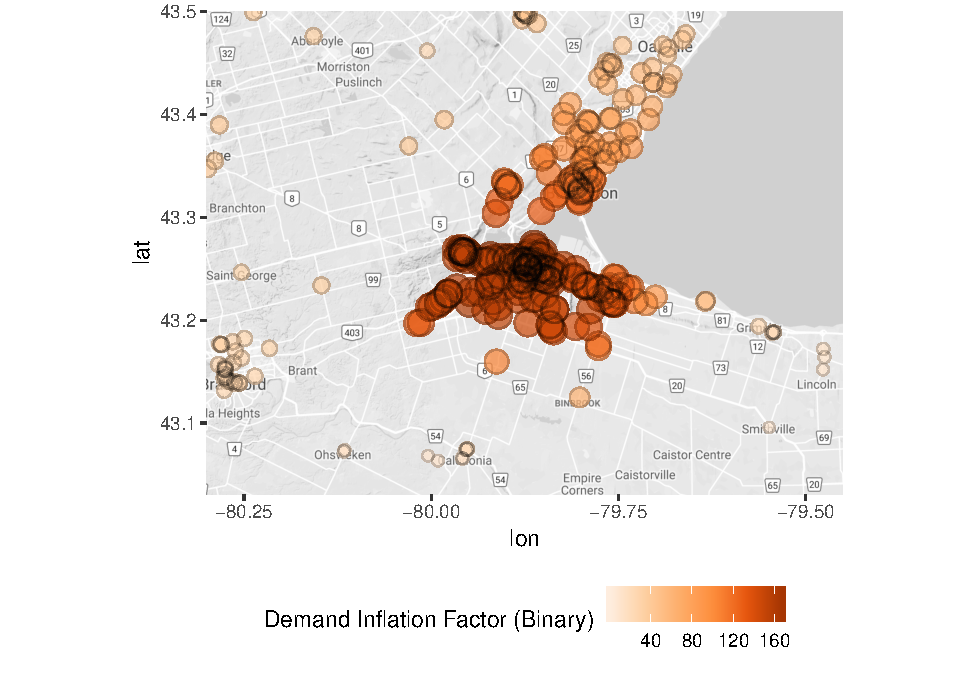
\includegraphics[width=0.95\linewidth]{Supply_and_Demand_Inflation_in_FCA_Methods_v2.0_files/figure-latex/fig10-map-demand-inflation-binary-1} \caption{\label{fig:fig10-map-demand-inflation-binary}Demand inflation, binary impedance function}\label{fig:fig10-map-demand-inflation-binary}
\end{figure}

\begin{figure}
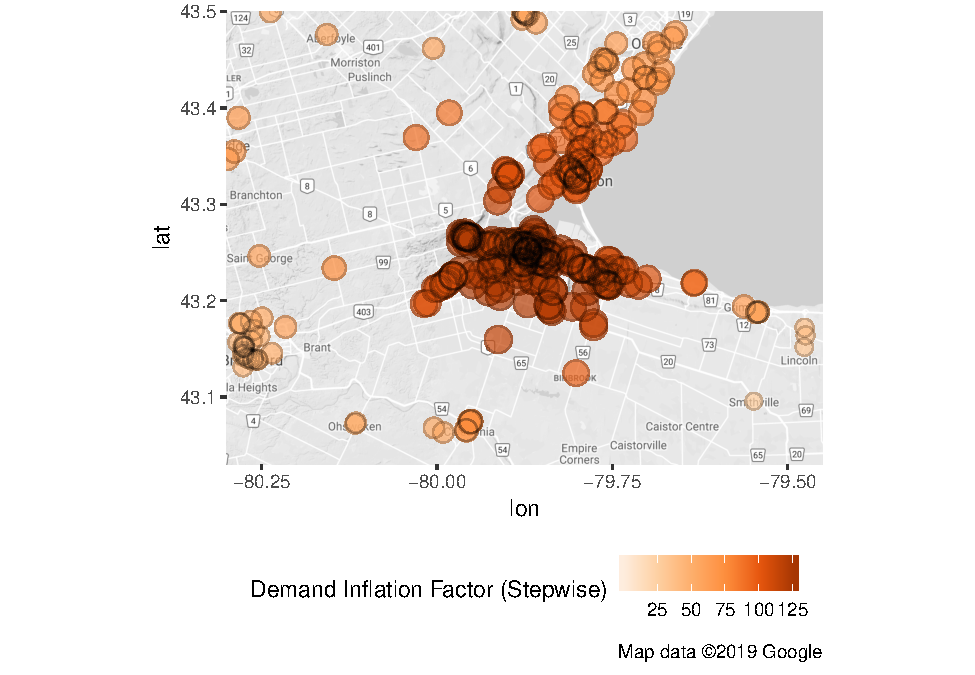
\includegraphics[width=0.95\linewidth]{Supply_and_Demand_Inflation_in_FCA_Methods_v2.0_files/figure-latex/fig11-map-demand-inflation-stepwise-1} \caption{\label{fig:fig11-map-demand-inflation-stepwise}Demand inflation, stepwise impedance function}\label{fig:fig11-map-demand-inflation-stepwise}
\end{figure}

The map of accessibility for the implementation of 2SFCA is shown in Fig
\ref{fig:fig12-map-accessibility-binary} and with the adjusted weights
for proportional allocation in Fig
\ref{fig:fig13-map-accessibility-binary-adjusted}. The general patterns
observed in the figures are as expected, with higher accessibility in
denser, better connected parts of the region. Relatively high
accessibility in the north and west of the CMA is due to proximity to
other major population centers such as Oakville, Kitchener, and
Waterloo. A question, however, is the degree of inflation of
accessibility in the original 2SFCA? Fig
\ref{fig:fig14-map-accessibility-binary-comparison} plots the ratio of
the binary and adjusted binary accessibility measures. Here it can be
seen that the unadjusted accessibility values are at least three times
greater than their adjusted counterparts within the study area. This
inflation, moreover, is not uniform across space, with inflation of the
binary accessibility values up to 8 times greater than those from the
adjusted model at the edges of the city where the 15-minute catchment
areas begin to overlap with neighboring municipalites.

\begin{figure}
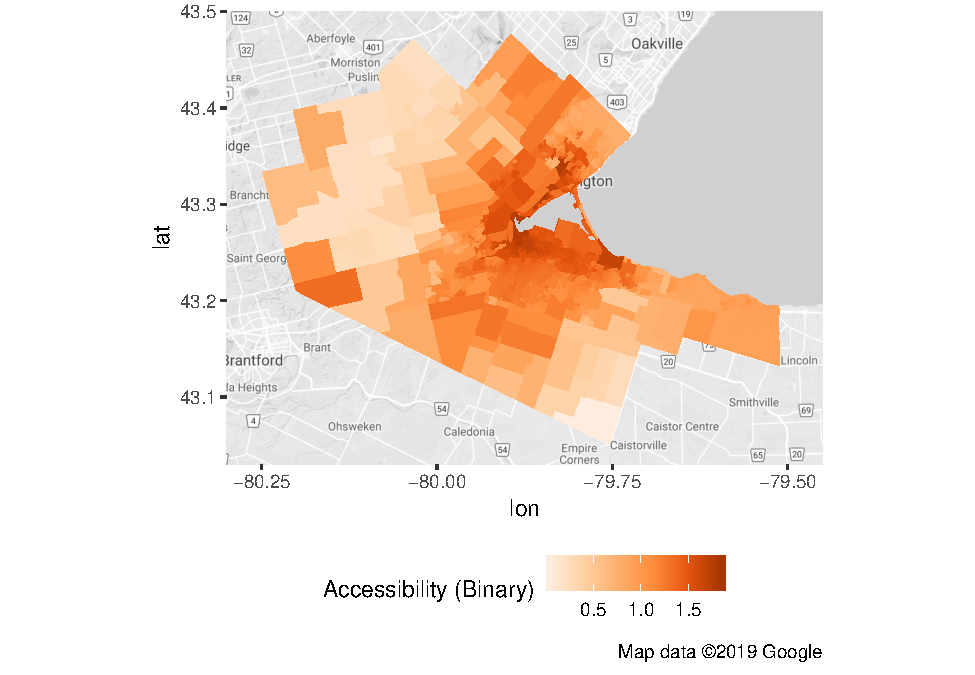
\includegraphics[width=0.95\linewidth]{Supply_and_Demand_Inflation_in_FCA_Methods_v2.0_files/figure-latex/fig12-map-accessibility-binary-1} \caption{\label{fig:fig12-map-accessibility-binary}Accessibility, binary impedance function}\label{fig:fig12-map-accessibility-binary}
\end{figure}

\begin{figure}
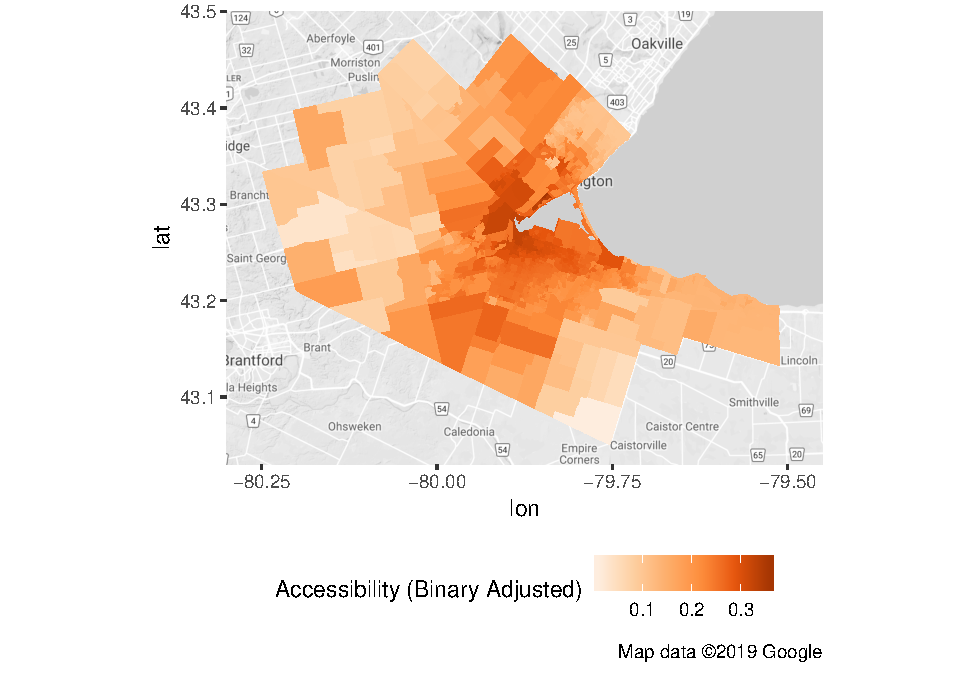
\includegraphics[width=0.95\linewidth]{Supply_and_Demand_Inflation_in_FCA_Methods_v2.0_files/figure-latex/fig13-map-accessibility-binary-adjusted-1} \caption{\label{fig:fig13-map-accessibility-binary-adjusted}Accessibility, adjusted binary impedance function}\label{fig:fig13-map-accessibility-binary-adjusted}
\end{figure}

\begin{figure}
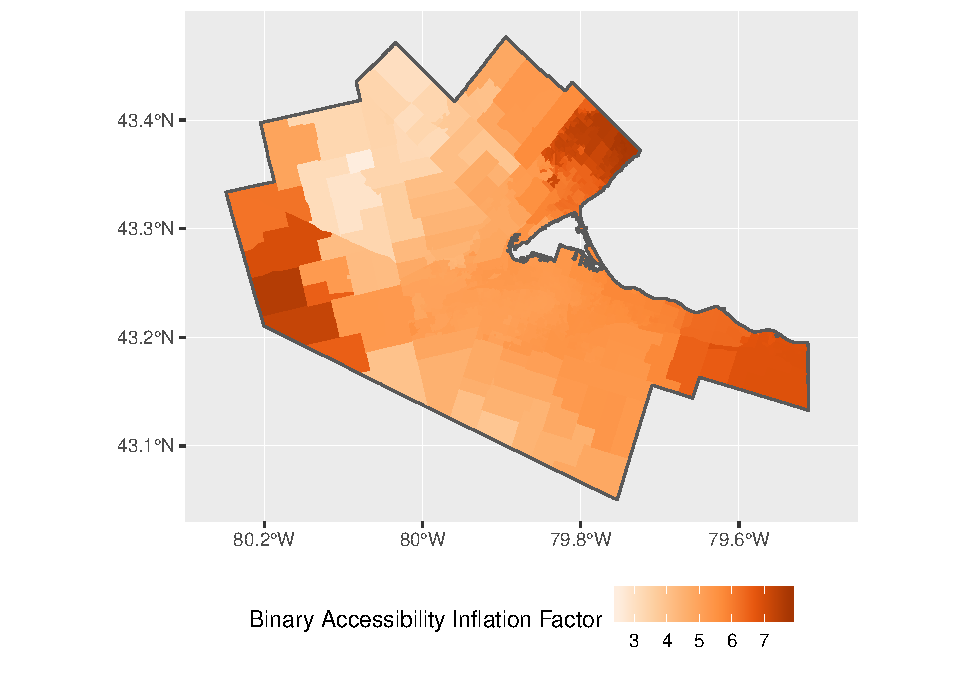
\includegraphics[width=0.95\linewidth]{Supply_and_Demand_Inflation_in_FCA_Methods_v2.0_files/figure-latex/fig14-map-accessibility-binary-comparison-1} \caption{\label{fig:fig14-map-accessibility-binary-comparison}Accessibility Inflation factor, binary impedance function}\label{fig:fig14-map-accessibility-binary-comparison}
\end{figure}

Why is this important? As noted by various authors {[}3,18{]}, in
traditional FCA methods, the sum of the population-weighted average of
accessibility across all population centers is equal to the regional
average provider-to-population ratio {[}18{]}. In the present case, the
weighted sum of accessibility in the unadjusted binary and stepwise
measures is 0.751. However, while this value is indeed identical to the
regional average provider-to-population ratio, it is problematic because
the share of the population correlates poorly with the pattern of
inflation observed (see Fig
\ref{fig:fig15-map-pop-share-inflation-comparison-binary}). The key
issue here is that accessibility is deflated by the share of the
population in a DA \(i\); however, the degree of inflation of demand and
supply depends not only of the population DA \(i\), but on the
population of every DA \(j\) with which DA \(i\) interacts via
overlapping catchment areas. As a consequence, deflating accessibility
using population shares in previous FCA methods does not accurately
offset demand and supply inflation.

\begin{figure}
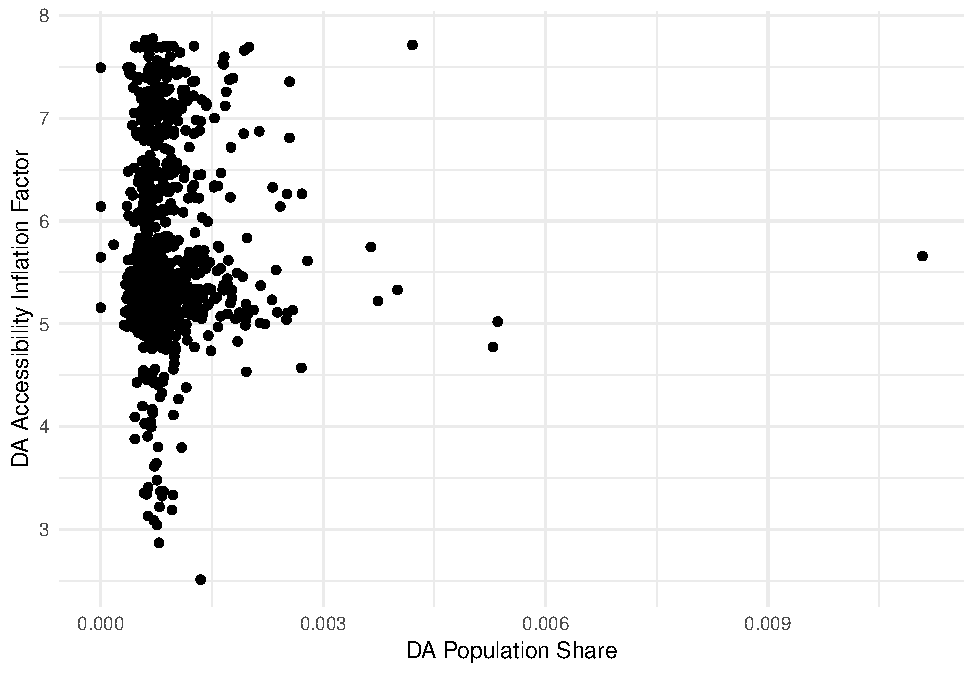
\includegraphics[width=0.95\linewidth]{Supply_and_Demand_Inflation_in_FCA_Methods_v2.0_files/figure-latex/fig15-map-pop-share-inflation-comparison-binary-1} \caption{\label{fig:fig15-map-pop-share-inflation-comparison-binary}Population share and inflation factors compared}\label{fig:fig15-map-pop-share-inflation-comparison-binary}
\end{figure}

Fig \ref{fig:fig16-map-accessibility-stepwise} and Fig
\ref{fig:fig17-map-accessibility-stepwise-adjusted} present the results
for the stepwise E2SFCA with and without the rectification. The results
are qualitatively similar to the 2FSCA, with the expected differences.
The inflation factor is even more substantial, given the larger
catchment areas used.

\begin{figure}
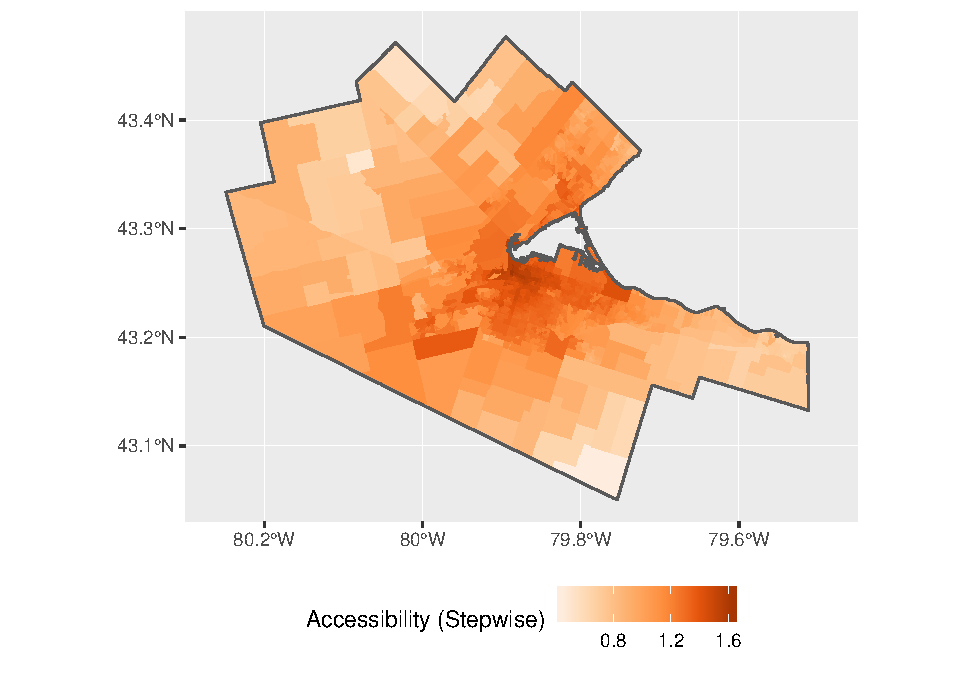
\includegraphics[width=0.95\linewidth]{Supply_and_Demand_Inflation_in_FCA_Methods_v2.0_files/figure-latex/fig16-map-accessibility-stepwise-1} \caption{\label{fig:fig16-map-accessibility-stepwise}Accessibility, stepwise impedance function}\label{fig:fig16-map-accessibility-stepwise}
\end{figure}

\begin{figure}
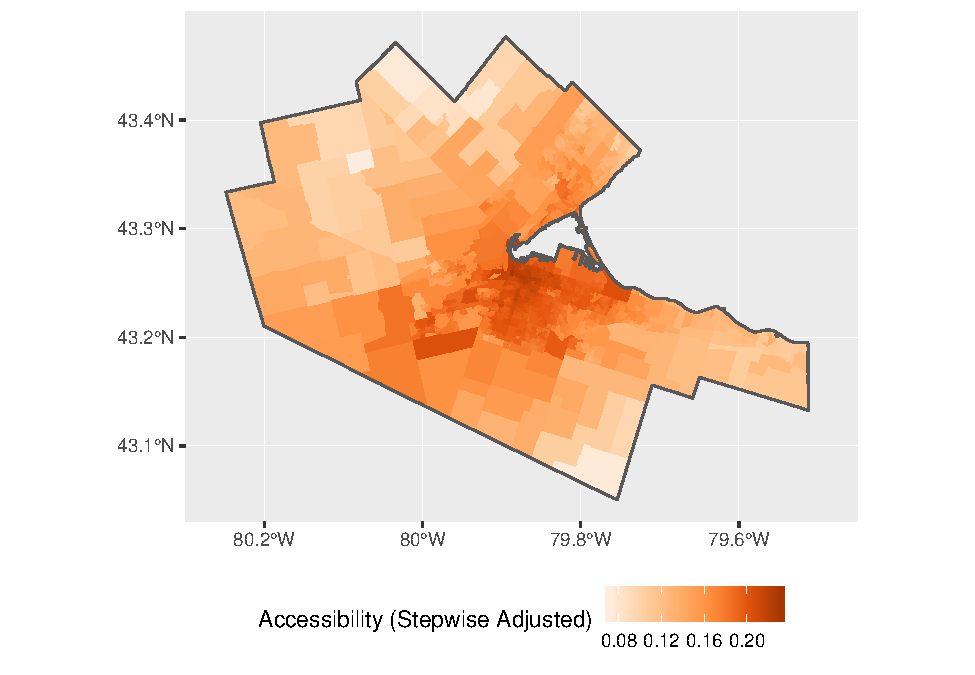
\includegraphics[width=0.95\linewidth]{Supply_and_Demand_Inflation_in_FCA_Methods_v2.0_files/figure-latex/fig17-map-accessibility-stepwise-adjusted-1} \caption{\label{fig:fig17-map-accessibility-stepwise-adjusted}Accessibility, adjusted stepwise impedance function}\label{fig:fig17-map-accessibility-stepwise-adjusted}
\end{figure}

\begin{figure}
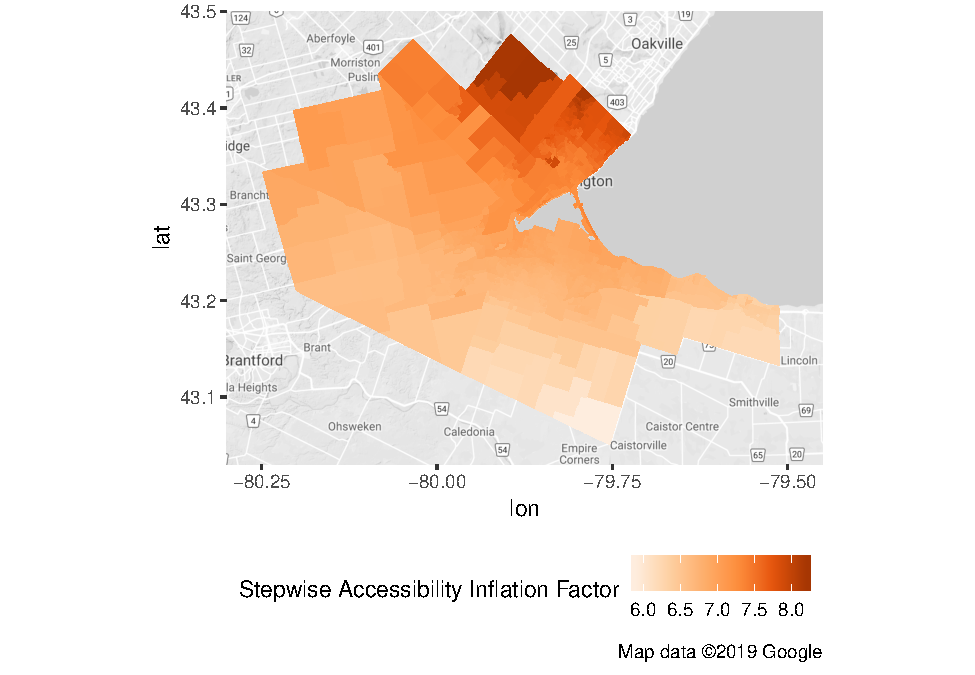
\includegraphics[width=0.95\linewidth]{Supply_and_Demand_Inflation_in_FCA_Methods_v2.0_files/figure-latex/fig18-map-accessibility-stepwise-comparison-1} \caption{\label{fig:fig18-map-accessibility-stepwise-comparison}Accessibility inflation factor, stepwise impedance function}\label{fig:fig18-map-accessibility-stepwise-comparison}
\end{figure}

\subsection{Disparity Analysis}\label{disparity-analysis}

An advantage of the use of adjusted weights for proportional allocation
of demand and level of service it that, after rectifying the inflation
artifact, they make it is possible to conduct accessibility disparity
analysis in a very intuitive way.

For instance, an analyst interested in equity analysis could allocate
the total level of service uniformly to every DA. In other words, the
total level of service (which equals the sum of accessibility over the
system) can be divided by the number of population centers in the system
to return the Average Local Population Center PPR. The resulting mean
value, call it \(L_i^e\) then would be assigned to the population
centers as their ``equitable'' share of the total level of service in
the system. Next, the equitative distribution of the level of service in
each population center is substracted from the estimated mean
accessibility to arrive at a disparity index. When the difference
between these two quantities is positive, this would indicate that a
DA's accessibility exceeds its equitable share of level of service. On
the other hand, when the difference is negative, the DA's accessibility
is below its equitable share of the level of service.

This approach is reminiscent of the Spatial Access Ratio (SPAR) proposed
by Wan et al. {[}28{]}, which is calculated as the ratio between a
population center's accessibility and the mean accessibility across all
population centers. Wan et al. {[}17{]} calculate SPAR based on the
results of their 3SFCA method, by rescaling the accessibility measures
to reflect the percentage difference in each population center's
accessibility relative to the mean. This measure is designed to overcome
the sensitivity of existing FCA metrics to the impedance function. In
contrast, the approach proposed here, enables more intuitive and
interpretable results by preserving the system-wide population and level
of service. In this way, a disparity index is useful to highlight the
absolute difference in accessible provider-to-population ratios across
population centers.

Disparity maps for the adjusted binary and stepwise impedance functions
are shown in Fig \ref{fig:fig19-map-disparities-binary} and Fig
\ref{fig:fig20-map-disparities-stepwise}. These figures reveal the
spatial distribution in disparity, with levels of access that are lower
than the mean in more rural parts of the city (where travel times are
longer and the distribution of physicians is more spatially disperse)
compared to levels of access that are greater than the mean in the
higher-density and more connected urban center.

\begin{figure}
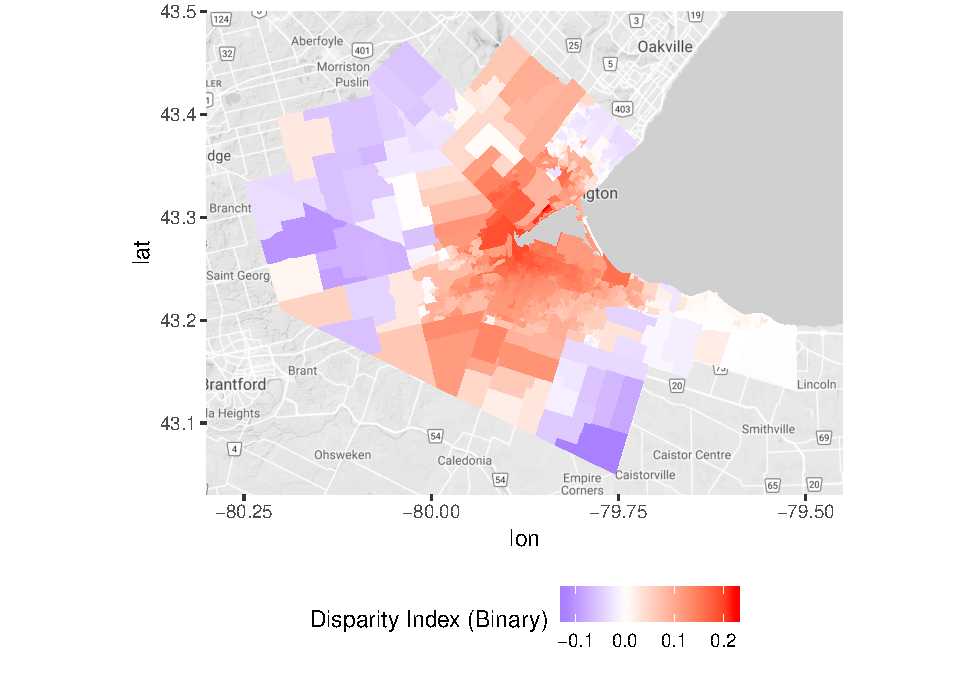
\includegraphics[width=0.95\linewidth]{Supply_and_Demand_Inflation_in_FCA_Methods_v2.0_files/figure-latex/fig19-map-disparities-binary-1} \caption{\label{fig:fig19-map-disparities-binary}Accessibility disparities, adjusted binary impedance function}\label{fig:fig19-map-disparities-binary}
\end{figure}

\begin{figure}
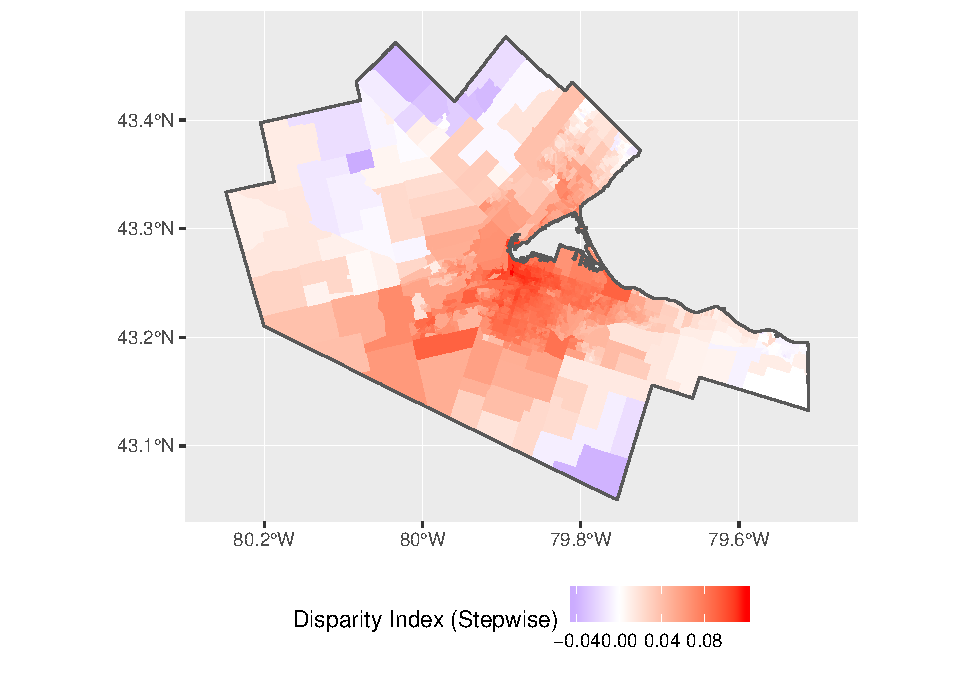
\includegraphics[width=0.95\linewidth]{Supply_and_Demand_Inflation_in_FCA_Methods_v2.0_files/figure-latex/fig20-map-disparities-stepwise-1} \caption{\label{fig:fig20-map-disparities-stepwise}Accessibility disparities, adjusted stepwise impedance function}\label{fig:fig20-map-disparities-stepwise}
\end{figure}

\section{Conclusion}\label{conclusion}

Accessibility to healthcare is an issue of continued interest in health
geography. One of the most popular approaches to estimating
accessibility is the 2SFCA method and its associated family of FCA
models due to their simplification of more complex gravity models and
their interpretation as proxies for provider-to-population ratios. These
properties make FCA approaches particularly appealing for health policy.
In this paper, we have argued that the overestimation of demand and
level of service in FCA approaches poses a challenge to the
interpretation of accessibility and the identification of spatial
disparities in access, with potentially deleterious consequences for
policy analysis.

The issue of overestimation of demand and level of service has been
recognized before, notably by Wan et al. {[}17{]} and Delamater
{[}18{]}, and alternative approaches have been proposed that seek to
offset or reduce the problem. Nevertheless, the present paper has shown
that the inflation of demand is present in all existing FCA methods.
Moreover, we also show that in some cases, demand is deflated, and
detail the potential for inflation/deflation on the supply side. To
overcome these issues, we draw from the fields of spatial statistics and
econometrics, to incorporate row-standardized impedance weights in the
calculation of demand, and column-standardized impedance weights to
adjust the level of service. These adjustments ensure that allocation of
demand and level of service are proportional. As a result, both the
system-wide population and level of service are preserved in the
estimation of accessibility.

The case study in Hamilton CMA reveals the extent of inflation in
accessibility inherent in the unadjusted approaches compared to the
adjusted binary and stepwise FCA methods. Furthermore, the adjustments
result in local provider-to-population ratios which can be easily
understood relative to the system-wide equitable level of service
through the calculation of a disparity index. The applicability of these
values is particularly enhanced by the use of a travel survey to inform
the estimated impedance functions. Taken together, these innovations
provide estimates of spatial accessibility and disparity that are robust
to the regional distribution of supply and demand, as well as observed
travel behaviour. By extension, these properties mean that the adjusted
approach employed here can offer more rigorous recommendations for
health policy.

Finally, 1) we proposed a set of slack factors to modulate the estimates
of demand and/or level of supply to account for system inefficiencies;
and 2) demonstrated the use of a disparity index to conduct equity
analysis.

In conclussion, the research presented in this paper demonstrates how a
relatively simple adjustment of the impedance weights can help to
overcome the inflation/deflation issue inherent in previous FCA
approaches. By incorporating these methods into the estimation of
accessibility to healthcare services, future research can help to ensure
that the FCA approach continues to live up to its promise as an
intuitive and policy-relevant method for investigating access and
disparity.

\section*{References}\label{references}
\addcontentsline{toc}{section}{References}

\hypertarget{refs}{}
\hypertarget{ref-Apparicio2017}{}
1. Apparicio P, Gelb J, Dube AS, Kingham S, Gauvin L, Robitaille E. The
approaches to measuring the potential spatial access to urban health
services revisited: Distance types and aggregation-error issues.
International Journal of Health Geographics. 2017;16.
doi:\href{https://doi.org/10.1186/s12942-017-0105-9}{10.1186/s12942-017-0105-9}

\hypertarget{ref-Joseph1982}{}
2. Joseph AE, Bantock PR. Measuring potential physical accessibility to
general practitioners in rural areas: A method and case study. Social
science \& medicine. Elsevier; 1982;16: 85--90.

\hypertarget{ref-Luo2003}{}
3. Luo W, Wang FH. Measures of spatial accessibility to health care in a
gis environment: Synthesis and a case study in the chicago region.
Environment and Planning B-Planning \& Design. 2003;30: 865--884.
Available:
\href{ISI:000187989500005\%0AC:/Papers/Environment\%20and\%20Planning\%20B/EPB\%20(2003)\%2030\%20(6)\%20865-885.pdf}{ISI:000187989500005
C:/Papers/Environment and Planning B/EPB (2003) 30 (6) 865-885.pdf}

\hypertarget{ref-Radke2000}{}
4. Radke J, Mu L. Spatial decomposition, modeling and mapping service
regions to predict access to social programs. Annals of Geographic
Information Sciences. 2000;6: 105--112.

\hypertarget{ref-Bauer2017}{}
5. Bauer J, Muller P, Maier W, Groneberg DA. Orthopedic workforce
planning in germany - an analysis of orthopedic accessibility. Plos One.
2017;12: 15.
doi:\href{https://doi.org/10.1371/journal.pone.0171747}{10.1371/journal.pone.0171747}

\hypertarget{ref-Kim2018}{}
6. Kim Y, Byon YJ, Yeo H. Enhancing healthcare accessibility
measurements using gis: A case study in seoul, korea. Plos One. 2018;13:
19.
doi:\href{https://doi.org/10.1371/journal.pone.0193013}{10.1371/journal.pone.0193013}

\hypertarget{ref-Fujita2017}{}
7. Fujita M, Sato Y, Nagashima K, Takahashi S, Hata A. Impact of
geographic accessibility on utilization of the annual health check-ups
by income level in japan: A multilevel analysis. Plos One. 2017;12: 14.
doi:\href{https://doi.org/10.1371/journal.pone.0177091}{10.1371/journal.pone.0177091}

\hypertarget{ref-Song2013}{}
8. Song PG, Zhu YJ, Mao X, Li Q, An L. Assessing spatial accessibility
to maternity units in shenzhen, china. Plos One. 2013;8: 7.
doi:\href{https://doi.org/10.1371/journal.pone.0070227}{10.1371/journal.pone.0070227}

\hypertarget{ref-McGrail2009}{}
9. McGrail MR, Humphreys JS. Measuring spatial accessibility to primary
care in rural areas: Improving the effectiveness of the two-step
floating catchment area method. Applied Geography. 2009;29: 533--541.
doi:\href{https://doi.org/10.1016/j.apgeog.2008.12.003}{10.1016/j.apgeog.2008.12.003}

\hypertarget{ref-Shah2016}{}
10. Shah TI, Bell S, Wilson K. Spatial accessibility to health care
services: Identifying under-serviced neighbourhoods in canadian urban
areas. Plos One. 2016;11.
doi:\href{https://doi.org/10.1371/journal.pone.0168208}{10.1371/journal.pone.0168208}

\hypertarget{ref-Luo2009}{}
11. Luo W, Qi Y. An enhanced two-step floating catchment area (e2sfca)
method for measuring spatial accessibility to primary care physicians.
Health \& Place. 2009;15: 1100--1107. Available:
\href{ISI:000270348400023\%0AC:/Papers/Health\%20and\%20Place/Health\%20and\%20Place\%20(2009)\%2015\%20(4)\%201100-1107.pdf}{ISI:000270348400023
C:/Papers/Health and Place/Health and Place (2009) 15 (4) 1100-1107.pdf}

\hypertarget{ref-Dai2010}{}
12. Dai D. Black residential segregation, disparities in spatial access
to health care facilities, and late-stage breast cancer diagnosis in
metropolitan detroit. Health \& place. Elsevier; 2010;16: 1038--1052.

\hypertarget{ref-Bauer2016}{}
13. Bauer J, Groneberg DA. Measuring spatial accessibility of health
care providers - introduction of a variable distance decay function
within the floating catchment area (fca) method. Plos One. 2016;11.
doi:\href{https://doi.org/10.1371/journal.pone.0159148}{10.1371/journal.pone.0159148}

\hypertarget{ref-Mao2013}{}
14. Mao L, Nekorchuk D. Measuring spatial accessibility to healthcare
for populations with multiple transportation modes. Health \& Place.
2013;24: 115--122.
doi:\href{https://doi.org/10.1016/j.healthplace.2013.08.008}{10.1016/j.healthplace.2013.08.008}

\hypertarget{ref-Ngui2011}{}
15. Ngui A, Apparicio P. Optimizing the two-step floating catchment area
method for measuring spatial accessibility to medical clinics in
montreal. Bmc Health Services Research. 2011;11. Available:
\url{http://www.biomedcentral.com/1472-6963/11/166}

\hypertarget{ref-Bell2013}{}
16. Bell S, Wilson K, Bissonnette L, Shah T. Access to primary health
care: Does neighborhood of residence matter? Annals of the Association
of American Geographers. Taylor \& Francis; 2013;103: 85--105.

\hypertarget{ref-Wan2012}{}
17. Wan N, Zou B, Sternberg T. A three-step floating catchment area
method for analyzing spatial access to health services. International
Journal of Geographical Information Science. 2012;26: 1073--1089.
doi:\href{https://doi.org/10.1080/13658816.2011.624987}{10.1080/13658816.2011.624987}

\hypertarget{ref-Delamater2013}{}
18. Delamater PL. Spatial accessibility in suboptimally configured
health care systems: A modified two-step floating catchment area
(m2sfca) metric. Health \& Place. 2013;24: 30--43.
doi:\href{https://doi.org/10.1016/j.healthplace.2013.07.012}{10.1016/j.healthplace.2013.07.012}

\hypertarget{ref-Luo2014}{}
19. Luo J. Integrating the huff model and floating catchment area
methods to analyze spatial access to healthcare services. Transactions
in GIS. Wiley Online Library; 2014;18: 436--448.

\hypertarget{ref-Taylor1971}{}
20. Taylor PJ. Distance transformation and distance decay functions.
Geographical Analysis. 1971;3: 221--238.
doi:\href{https://doi.org/doi:10.1111/j.1538-4632.1971.tb00364.x}{doi:10.1111/j.1538-4632.1971.tb00364.x}

\hypertarget{ref-Kwan1998}{}
21. Kwan MP. Space-time and integral measures of individual
accessibility: A comparative analysis using a point-based framework.
Geographical Analysis. 1998;30: 191--216. Available:
\href{ISI:000074579200001\%0AC:/Papers/Geographical\%20Analysis/Geographical\%20Analysis\%20(1998)\%2030\%20(3)\%20191-216.pdf}{ISI:000074579200001
C:/Papers/Geographical Analysis/Geographical Analysis (1998) 30 (3) 191-216.pdf}

\hypertarget{ref-Schuurman2010}{}
22. Schuurman N, Berube M, Crooks VA. Measuring potential spatial access
to primary health care physicians using a modified gravity model.
Canadian Geographer-Geographe Canadien. 2010;54: 29--45.
doi:\href{https://doi.org/10.1111/j.1541-0064.2009.00301.x}{10.1111/j.1541-0064.2009.00301.x}

\hypertarget{ref-Tobler1979}{}
23. Tobler WR. Smooth pycnophylactic interpolation for geographical
regions. Journal of the American Statistical Association. 1979;74:
519--530. Available:
\href{ISI:A1979HS22400001\%0AC:/Papers/Journal\%20of\%20the\%20American\%20Statistical\%20Association/Journal\%20of\%20the\%20American\%20Statistical\%20Association\%20(1979)\%2074\%20(367)\%20519-530.pdf}{ISI:A1979HS22400001
C:/Papers/Journal of the American Statistical Association/Journal of the American Statistical Association (1979) 74 (367) 519-530.pdf}

\hypertarget{ref-Anselin1988}{}
24. Anselin L. Spatial econometrics: Methods and models. Dordrecht:
Kluwer; 1988.

\hypertarget{ref-Griffith1988}{}
25. Griffith DA. Advanced spatial statistics: Special topics in the
exploration of quantitative spatial data series. Dordrecht: Kluwer;
1988.

\hypertarget{ref-Ontario1991}{}
26. 1991, Medicine Act, S.O. 1991, c. 30.

\hypertarget{ref-CIHI2018}{}
27. Health Information CI for. Number of physicians by
province/territory and specialty. Canadian Institute for Health
Information; 2018;

\hypertarget{ref-Wan2012SPAR}{}
28. Wan N, Zhan FB, Zou B, Chow E. A relative spatial access assessment
approach for analyzing potential spatial access to colorectal cancer
services in texas. Applied Geography. Elsevier; 2012;32: 291--299.

\nolinenumbers


\end{document}

